% !TeX root = ../../Book1.tex
% 纲要标题：## 附录 C　几何计算与图示
% 纲要位置：几何学计划纲要.md，第 966 行。
% 正文状态：初稿；尚未正式审核。

% 纲要内容开始
% 
% > 图示服务于局部图、变换和不变量的核验，不以软件输出代替证明。
% 
% * **坐标、符号与可验证计算**
%   * 图册覆盖范围和坐标奇点
%   * 联络、曲率及 Bianchi 核验
%   * 参数模型、精确恒等式与误差界
% 
% * **数值误差与几何解释**
% 
%   区分几何退化、坐标退化和离散化误差；记录度量、法向、取向、步长与精度，使计算能够独立复核。
% 
% ---
% 
% 纲要内容结束

\chapter{几何计算与图示}
\label{g1:app:C}
\BookChapterNumber{g1:app:C}

\begin{chapterabstract}
	同一个几何对象可以在一张坐标图中表现为规则的公式，在另一张图中出现发散系数或退化矩阵。计算的任务首先是辨认这些表示的定义域与变换规律，再判断数值结果究竟说明了什么。本附录从球面的经纬参数和立体投影图出发，核对覆盖、取向与度量；随后计算联络、曲率及 Bianchi 恒等式，并用旋转椭球展示参数条件、精确恒等式和法向误差界。最后通过中心差分的误差分析与球面曲率实验，区分几何退化、坐标失效、截断误差及输入误差，使图示与数值能够服务于可复核的几何论证。
\end{chapterabstract}

\begin{learninggoals}
	\begin{itemize}
		\item 写出球面坐标图的准确覆盖范围、逆映射和过渡映射，识别经纬参数在极点的失效。
		\item 在坐标或标架变化后核对度量、法向、联络及曲率的变换，而不直接比较不具不变意义的系数。
		\item 展开一个非交换矩阵值联络的曲率与 Bianchi 核验，说明恒等式核验的适用范围。
		\item 对旋转椭球计算基本形式和曲率，给出参数条件及有限代数证书。
		\item 从输入误差和正则性下界推导法向与差分误差，说明步长和精度为何需要共同选择。
		\item 记录数值实验的对象、度量、取向、离散公式及误差依据，区分有限观测和已证结论。
	\end{itemize}
\end{learninggoals}

单位球面在经纬参数中的度量为 \(\mathrm{d}\theta^2+\sin^2\theta\,\mathrm{d}\phi^2\)。当 \(\theta\) 趋近零时，一个系数趋于零，逆矩阵中的相应系数趋于无穷；若只绘制这些系数，很容易把北极误认为曲面的奇点。然而北极附近可以写成光滑图像 \(z=\sqrt{1-x^2-y^2}\)，球面的曲率在那里仍然等于 \(1\)。两个公式描述的是同一个几何对象，出现差别的原因必须在坐标及其适用范围中寻找。

\ProseParagraphBreak

计算中还会出现更隐蔽的问题：一个曲率表达式在许多测试点上都给出正确数值，仍可能在遗漏的参数范围内失效；将一个恒等式的两边相减后得到零，也可能只是因为受维数限制，其中的高次微分形式都为零。因而需要把三种论据分清。精确推导说明公式为何成立，数值实验揭示特定输入下的表现，误差界则把有限精度的数据与连续几何量联系起来。图示呈现覆盖范围和局部模型。

\ProseParagraphBreak

本附录使用\secref{g1:sec:0801}的正则参数曲面与第一基本形式、\secref{g1:sec:0802}的形算子及曲率公式，以及\chapref{g1:ch:11}的坐标图与光滑过渡。联络计算另需\chapref{g1:ch:14}的外微分、楔积和\chapref{g1:ch:15}的局部联络矩阵；下文会重述所用约定。尚未学习联络的读者可以先读图册、参数模型和数值实验，再回到中间的小节。所选例子都给出可直接重算的公式，不要求使用某一种计算软件。

\section{坐标、符号与可验证计算}
\label{g1:sec:C01}

要比较两次计算，先要知道两次计算是否表示同一个点、同一个切向量及同一个法向。坐标图给出定义域和点的对应，度量与标架决定分量的意义，参数条件则保证求逆和归一化合法。本节把这些问题放进具体模型中：先计算球面图册，再处理联络中的非交换乘法，最后把一个曲面族的精确公式转化为带条件的误差估计。

\subsection{图册覆盖范围和坐标奇点}
\label{g1:subsec:C01:01}

球面的经线在两极汇合。把经纬网格画得更密，并不能在极点区分经度方向；但极点附近的球面仍是一块光滑曲面。计算中看到分母趋零、度量矩阵退化或许多参数点具有同一个像时，首先要查的是当前参数表示的定义域与逆映射。只有明确了这些范围，公式才能用于判断几何对象。

\ProseParagraphBreak

回顾\cref{g1:def:smooth-manifold}：坐标图是流形中一个开集 \(U\) 到Euclid 开集 \(D\) 的同胚 \(\varphi:U\rightarrow D\)，而计算曲面时写出的参数通常是相反方向的 \(\Phi=\varphi^{-1}:D\rightarrow U\)。因此，给出 \(\Phi\) 的表达式后，仍须确定 \(D\)、像 \(U\)、单射性及逆映射的光滑性。若要用若干张图描述整个对象，还须核对这些 \(U\) 的并是否覆盖它。

\begin{proposition}[由参数取得坐标图]
	\label{g1:prop:parameter-chart-test}
	设 \(M\) 是已给定光滑结构的二维无边界流形，\(D\subset\mathbb R^2\) 是开集，\(\Phi:D\rightarrow M\) 光滑。若 \(\Phi\) 单射，且对每个 \(a\in D\)，\(\mathrm{d}\Phi_a:\mathbb R^2\rightarrow\mathrm{T}_{\Phi(a)}M\) 的秩均为 \(2\)，则 \(U=\Phi(D)\) 是 \(M\) 的开集，\(\Phi:D\rightarrow U\) 是微分同胚，\((U,\Phi^{-1})\) 是一张光滑坐标图。
\end{proposition}
\begin{proof}
	源、目标的维数都为 \(2\)，所以满秩微分是线性同构。由\cref{g1:thm:inverse-function}，每个 \(a\in D\) 都有一个开邻域 \(D_a\)，使 \(\Phi\) 把它微分同胚地映到 \(M\) 的一个开集 \(U_a\)。因此 \(U=\bigcup_{a\in D}U_a\) 开。全局单射性保证各局部逆在交叠处给出同一个原像，因而粘成 \(U\) 上的逆映射。该逆映射在每个 \(U_a\) 上光滑，所以在 \(U\) 上光滑。
\end{proof}

满秩保证局部可逆，单射性进一步排除不同参数分支映到同一点；两者结合，便在像 \(U\) 上得到一张图。它覆盖的范围由参数像决定，可能小于整个 \(M\)。同一球面参数可以同时展示这三项条件的作用。

\ProseParagraphBreak

令 \(S^2=\{(x,y,z):x^2+y^2+z^2=1\}\)，赋予\cref{g1:exm:sphere-smooth-atlas}中的标准光滑结构。取余纬 \(\theta\) 和经度 \(\phi\)，定义
\begin{equation}
	\label{g1:eq:spherical-chart-parameters}
	\Phi(\theta,\phi)
	=(\sin\theta\cos\phi,\sin\theta\sin\phi,\cos\theta),
	\qquad 0<\theta<\pi,\quad-\pi<\phi<\pi.
\end{equation}
这里纬度等于 \(\pi/2-\theta\)；采用余纬是为了使北极对应 \(\theta=0\)。经度区间的两端不包括在内，是为了避免 \(-\pi\) 与 \(\pi\) 表示同一条经线。

\begin{proposition}[经纬图的精确范围]
	\label{g1:prop:spherical-chart-domain}
	设 \(S^2\subset\mathbb R^3\) 为带标准光滑结构及诱导度量的单位球面，定义
	\[
		\Phi(\theta,\phi)=(\sin\theta\cos\phi,\sin\theta\sin\phi,\cos\theta),
		\qquad (\theta,\phi)\in(0,\pi)\times(-\pi,\pi).
	\]
	令
	\[
		\Gamma=\{(x,y,z)\in S^2:y=0,\ x\le0\},\qquad
		U=S^2\setminus\Gamma.
	\]
	则 \(\Phi\) 把开矩形 \((0,\pi)\times(-\pi,\pi)\) 微分同胚地映到 \(U\)。其诱导度量为
	\begin{equation}
		\label{g1:eq:spherical-chart-metric}
		g=\mathrm{d}\theta^2+\sin^2\theta\,\mathrm{d}\phi^2.
	\end{equation}
	若把同一三角函数表达式延伸到 \(\theta=0\) 或 \(\theta=\pi\)，其微分在这些参数处的秩降为 \(1\)。
\end{proposition}
\begin{proof}
	集合 \(\Gamma\) 是一条包含两极的闭半经线，所以 \(U\) 在球面中开。对 \(p=(x,y,z)\in U\)，令 \(\rho=\sqrt{x^2+y^2}\)。此时 \(\rho>0\)，并且 \(\rho+x>0\)：等号只能发生在 \(y=0,x\le0\) 的被删去部分。于是可定义
	\[
		\theta=\arccos z,\qquad
		\phi=2\arctan\frac{y}{\rho+x}.
	\]
	第一项落在 \((0,\pi)\)，第二项落在 \((-\pi,\pi)\)。半角公式给出 \(\cos\phi=x/\rho\)、\(\sin\phi=y/\rho\)，而 \(\sin\theta=\rho\)，所以代回得到 \(\Phi(\theta,\phi)=p\)。反过来，原参数区间中 \(\cos\theta\) 唯一确定 \(\theta\)，经度在这个长度为 \(2\pi\) 的开区间内也唯一，故所给反解确为逆映射。\(\arccos\) 在 \((-1,1)\) 上光滑，平方根和分式在所列范围内光滑，因此逆映射光滑，原映射也光滑。

	直接求导得
	\[
		\begin{aligned}
			\Phi_\theta&=(\cos\theta\cos\phi,\cos\theta\sin\phi,-\sin\theta),\\
			\Phi_\phi&=(-\sin\theta\sin\phi,\sin\theta\cos\phi,0).
		\end{aligned}
	\]
	两个向量正交，长度分别为 \(1\) 与 \(\sin\theta\)，故在开矩形内线性无关，第一基本形式就是\eqref{g1:eq:spherical-chart-metric}。在 \(\theta=0,\pi\) 处，\(\Phi_\phi=0\)，而 \(\Phi_\theta\) 仍为单位向量，所以延伸后的参数映射秩为 \(1\)。
\end{proof}

这张图漏掉的不只是两个极点，还漏掉整条选作经度割线的半经线。在 \(0<\theta<\pi\)、\(\phi=\pm\pi\) 处，三角函数表达的微分仍满秩；问题是两端重复表示同一点，因而不能把包含两端的矩形直接当作一张Euclid 开集坐标图。把割线移到另一条经线，可以覆盖这些非极点。两极则不同：所有经度在同一极点汇合，必须改用另一种参数。

\ProseParagraphBreak

度量矩阵 \(\operatorname{diag}(1,\sin^2\theta)\) 在 \(\theta=0\) 的退化，恰好来自 \(\Phi_\phi=0\)。它是在一个已经不再浸入的映射下拉回度量所得的退化形式，不能当作极点处的有效坐标矩阵。我们把这类由表示方式造成的失效称为\term[zuobiaoqidian]{坐标奇点}[coordinate singularity]；下面换图后，极点处的度量仍是正定的。

\ProseParagraphBreak

取北极 \(N=(0,0,1)\)、南极 \(S=(0,0,-1)\)。\cref{g1:ex:stereographic-smooth-charts}已经给出一般球面的立体投影；这里重述二维公式，并把覆盖范围和度量计算连在一起。以下按投影中心命名两张图，记
\[
	U_N=S^2\setminus\{N\},\qquad U_S=S^2\setminus\{S\},
\]
并定义
\[
	\sigma_N(x,y,z)=\frac{(x,y)}{1-z},\qquad
	\sigma_S(x,y,z)=\frac{(x,y)}{1+z}.
\]
例如，从 \(N\) 到 \(p\ne N\) 的直线与平面 \(z=0\) 相交，交点的前两坐标就是 \(\sigma_N(p)\)。这张图删除投影中心 \(N\)，却完整包含 \(S\)。

\begin{proposition}[两张立体投影图及其度量]
	\label{g1:prop:stereographic-chart-metric}
	设 \(S^2\subset\mathbb R^3\) 为标准光滑单位球面，\(N=(0,0,1)\)、\(S=(0,0,-1)\)，\(U_N=S^2\setminus\{N\}\)、\(U_S=S^2\setminus\{S\}\)。定义 \(\sigma_N(x,y,z)=(x,y)/(1-z)\)、\(\sigma_S(x,y,z)=(x,y)/(1+z)\)。则 \(\sigma_N:U_N\to\mathbb R^2\)、\(\sigma_S:U_S\to\mathbb R^2\) 是光滑坐标图，并且 \(U_N\cup U_S=S^2\)。对 \(u=(u_1,u_2)\)，它们的逆映射分别为
	\begin{align}
		\Phi_N(u)&=\left(\frac{2u_1}{1+|u|^2},\frac{2u_2}{1+|u|^2},\frac{|u|^2-1}{1+|u|^2}\right),
		\label{g1:eq:stereographic-north-inverse}\\
		\Phi_S(u)&=\left(\frac{2u_1}{1+|u|^2},\frac{2u_2}{1+|u|^2},\frac{1-|u|^2}{1+|u|^2}\right).
		\label{g1:eq:stereographic-south-inverse}
	\end{align}
	在交叠区域中，过渡映射为
	\begin{equation}
		\label{g1:eq:stereographic-real-transition}
		\tau(u)=(\sigma_S\circ\Phi_N)(u)=\frac{u}{|u|^2},
		\qquad u\in\mathbb R^2\setminus\{0\},
	\end{equation}
	且 \(\tau^{-1}=\tau\)。单位球面的诱导度量在两张图中均为
	\begin{equation}
		\label{g1:eq:stereographic-sphere-metric}
		g=\frac{4}{(1+u_1^2+u_2^2)^2}
		\bigl(\mathrm{d}u_1^2+\mathrm{d}u_2^2\bigr).
	\end{equation}
\end{proposition}
\begin{proof}
	先解 \(u=(x,y)/(1-z)\)。球面方程给出
	\[
		|u|^2(1-z)^2=1-z^2=(1-z)(1+z).
	\]
	在 \(U_N\) 上 \(1-z\ne0\)，约去后得到 \(z=(|u|^2-1)/(1+|u|^2)\)，再代回 \((x,y)=(1-z)u\)，便得\eqref{g1:eq:stereographic-north-inverse}。该式对所有 \(u\in\mathbb R^2\) 有定义，像的第三坐标严格小于 \(1\)，直接代回两式得到两个复合恒等映射。将 \(z\) 换成 \(-z\) 得到另一张图及其逆。两图的坐标函数都是在分母非零处定义的光滑函数；逆式是分母始终为正的有理式。与第11章半球图比较时，只需在这些表达式中删除一个坐标，或把半球图的光滑平方根反解代入其中，所以它们与标准球面图册光滑相容。

	两个删去的点不同，故两图覆盖球面。在 \(\Phi_N\) 中，\(u=0\) 对应 \(S\)，恰是另一张图所删除的点。因此交叠的参数域是 \(\mathbb R^2\setminus\{0\}\)。将 \(\Phi_N\) 代入 \(\sigma_S\)，得到 \(u/|u|^2\)；再次应用同一个式子恢复 \(u\)，所以正逆过渡均光滑。

	最后计算度量。令 \(q=1+|u|^2\)，对参数向量 \(h\in\mathbb R^2\)，记 \(a=\langle u,h\rangle\)。微分为
	\[
		\mathrm{d}\Phi_N(u)[h]
		=\left(\frac{2h}{q}-\frac{4au}{q^2},\frac{4a}{q^2}\right).
	\]
	因此
	\[
		\left|\mathrm{d}\Phi_N(u)[h]\right|^2
		=\frac{4|h|^2}{q^2}-\frac{16a^2}{q^3}
		+\frac{16a^2(|u|^2+1)}{q^4}
		=\frac{4|h|^2}{q^2}.
	\]
	这给出\eqref{g1:eq:stereographic-sphere-metric}。\(\Phi_S\) 的最后一个微分分量只差负号，平方范数不变，所以它给出相同形式的度量矩阵。
\end{proof}

\begin{figure}[htbp]
	\centering
	% !TeX root = ../Book1.tex
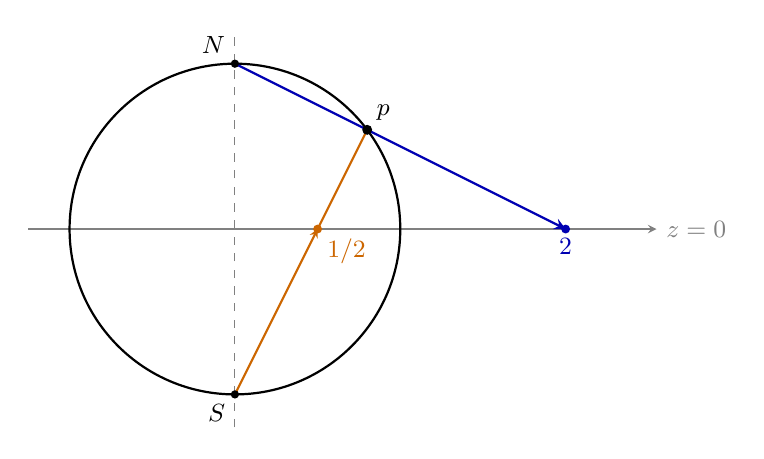
\begin{tikzpicture}[>=stealth,font=\small,x=2.1cm,y=2.1cm]
	\draw[gray,->] (-1.25,0)--(2.55,0) node[right] {\(z=0\)};
	\draw[gray,dashed] (0,-1.2)--(0,1.2);
	\draw[thick] (0,0) circle (1);
	\draw[blue!70!black,thick,->] (0,1)--(2,0);
	\draw[orange!80!black,thick] (0,-1)--(.8,.6);
	\draw[orange!80!black,->] (0,-1)--(.5,0);
	\fill (0,1) circle (1.5pt) node[above left] {\(N\)};
	\fill (0,-1) circle (1.5pt) node[below left] {\(S\)};
	\fill (.8,.6) circle (1.8pt) node[above right] {\(p\)};
	\fill[blue!70!black] (2,0) circle (1.6pt) node[below] {\(2\)};
	\fill[orange!80!black] (.5,0) circle (1.6pt) node[below right] {\(1/2\)};
\end{tikzpicture}

	\caption[两张立体投影图的覆盖]{在 \(y=0\) 的子午截面中，点 \(p=(4/5,0,3/5)\) 从北极、南极向赤道平面投影，所得横坐标分别为 \(2\) 与 \(1/2\)。两条直线显示投影中心与交点的关系；靠近北极时，南极投影仍给出接近零的有限坐标。}
	\label{g1:fig:stereographic-chart-coverage}
\end{figure}

两张图中的零坐标代表不同的点：\(\Phi_N(0)=S\)，\(\Phi_S(0)=N\)。在这两个点，度量矩阵都是 \(4I_2\)，正定而无退化。过渡式在 \(u=0\) 未定义，原因是对应点不属于两图的交集。

\ProseParagraphBreak

还可以把经纬表达与这两张图直接对照。在 \(0<\theta<\pi\) 内，半角公式给出
\[
	\begin{aligned}
		\sigma_N(\Phi(\theta,\phi))
		&=\cot\frac\theta2\,(\cos\phi,\sin\phi),\\
		\sigma_S(\Phi(\theta,\phi))
		&=\tan\frac\theta2\,(\cos\phi,\sin\phi).
	\end{aligned}
\]
当 \(\theta\to0\) 时，第一组坐标的模趋于无穷，而第二组趋于 \(0\)。球面上的点只是趋向北极，并没有在球面上趋向无穷远；发散的是一张删去北极的图中的坐标。与此同时，第二组是平面中的极坐标形式，\(\tan(\theta/2)=0\) 时所有经度给出同一个平面原点，这又解释了经纬参数的秩为何下降。

\ProseParagraphBreak

实际需要有限范围内的坐标时，可以在 \(z\ge0\) 采用 \(\sigma_S\)，在 \(z\le0\) 采用 \(\sigma_N\)。前一情形有
\[
	|\sigma_S(p)|^2=\frac{x^2+y^2}{(1+z)^2}
	=\frac{1-z}{1+z}\le1,
\]
后一情形同理有 \(|\sigma_N(p)|\le1\)。这些半球规定选图的规则，各张图仍使用原来的开图域。在选出的坐标值处，\eqref{g1:eq:stereographic-sphere-metric}满足
\[
	|h|^2\le g_u(h,h)\le4|h|^2.
\]
因此两张图足以把整个球面的计算安排在坐标模不超过 \(1\) 的区域内；在赤道附近二者都可使用，并由过渡式比较结果。

\begin{example}[参数秩下降而像集光滑]
	\label{g1:exm:cubic-plane-parametrization}
	映射
	\[
		F:\mathbb R^2\longrightarrow\mathbb R^3,\qquad
		F(s,t)=(s^3,t,0)
	\]
	是到整个平面 \(P=\{z=0\}\) 的连续双射，逆映射为 \((x,y,0)\mapsto(\sqrt[3]{x},y)\)，所以它还是同胚。但其微分的两列为 \((3s^2,0,0)\)、\((0,1,0)\)，在 \(s=0\) 时秩为 \(1\)，拉回Euclid 度量为
	\[
		F^*g=9s^4\,\mathrm{d}s^2+\mathrm{d}t^2.
	\]
	参数映射的微分将这个退化方向映成了零向量。平面本身仍有处处正则的参数 \((x,y)\mapsto(x,y,0)\)；问题在于原来的逆含有在零点不可微的立方根。因而 \((s,t)\) 不能作为标准光滑平面在该直线附近的光滑坐标。这把\cref{g1:exm:cubic-rank-change}中的一维现象放到了一个像集完全明确的曲面上。
\end{example}

要判断参数公式给出的对象，可以先确定其像，再寻找该像附近有效的坐标或正则定义方程。对球面，方程 \(H(x,y,z)=x^2+y^2+z^2-1=0\) 的微分在每个球面点都非零，\cref{g1:thm:regular-level-set}给出二维光滑水平集；对上例平面，定义方程 \(z=0\) 同样处处正则。因此，可以分别检查参数映射是否降秩，以及像集本身是否光滑。

\subsection{联络、曲率及 Bianchi 核验}
\label{g1:subsec:C01:02}

一份联络计算中，矩阵的行列次序、微分形式的楔积次序和坐标标架的选择会同时影响结果。例如，平直Euclid 平面在极坐标正交标架中已有非零联络矩阵；另一方面，一组常值矩阵也可能由于不交换而产生非零曲率。因此，核验应从“这组矩阵表示哪个标架中的哪一个联络”开始，再比较曲率定义、结构方程和恒等式。本小节把这些关系放进可逐项重算的模型中。

\ProseParagraphBreak

先固定\cref{g1:prop:connection-local-data}的约定。对秩 \(m\) 的实光滑向量丛，局部标架写为行 \(e=(e_1,\ldots,e_m)\)，截面写为 \(s=eu\)，其中 \(u\) 是列分量。联络矩阵 \(A\) 的第 \(j\) 列记录 \(\nabla e_j\)，即
\[
	\nabla e=eA,\qquad \nabla(eu)=e(\mathrm{d}u+Au).
\]
若 \(e'=eg\)，则同一截面的分量满足 \(u=gu'\)。对 \(eg\) 使用乘积法则，
\[
	\nabla(eg)=e(Ag+\mathrm{d}g)
	=e'g^{-1}(Ag+\mathrm{d}g),
\]
所以新矩阵为
\[
	A'=g^{-1}Ag+g^{-1}\mathrm{d}g.
\]
这里的附加项来自标架本身随位置变化。只有比较同一个联络时，才可以把两组局部矩阵放进这个公式。

\ProseParagraphBreak

矩阵值形式的乘积同时保留矩阵乘法与楔积。例如
\[
	(A\wedge A)^a{}_b=\sum_c A^a{}_c\wedge A^c{}_b.
\]
若在坐标中写 \(A=\sum_i A_i\,\mathrm{d}x^i\)，则把 \((i,j)\) 与 \((j,i)\) 两项合并，得到
\[
	A_iA_j\,\mathrm{d}x^i\wedge\mathrm{d}x^j
	+A_jA_i\,\mathrm{d}x^j\wedge\mathrm{d}x^i
	=[A_i,A_j]\,\mathrm{d}x^i\wedge\mathrm{d}x^j.
\]
因此\cref{g1:thm:curvature-structure-equation}给出的曲率具体为
\begin{equation}\label{g1:eq:connection-check-curvature-components}
	F=\mathrm{d}A+A\wedge A
	=\sum_{i<j}F_{ij}\,\mathrm{d}x^i\wedge\mathrm{d}x^j,
	\qquad F_{ij}=\partial_iA_j-\partial_jA_i+[A_i,A_j].
\end{equation}
这里对 \(i<j\) 求和，不另乘 \(1/2\)。并且 \(R(X,Y)(eu)=eF(X,Y)u\)，其中
\[
	R(X,Y)s=\nabla_X\nabla_Ys-\nabla_Y\nabla_Xs-\nabla_{[X,Y]}s.
\]
这个作用公式使矩阵中的正负号最终可以用一个实际的纤维向量来校准。

\ProseParagraphBreak

在曲率二形式上，本小节将自同态丛的外协变微分简记为
\[
	\mathrm{D}F=\mathrm{d}F+A\wedge F-F\wedge A.
\]
最后一项的负号来自\eqref{g1:eq:endomorphism-exterior-derivative}中二次形式的偶数次数。\cref{g1:thm:bianchi-identity}已证明，对由 \(A\) 计算出的曲率总有 \(\mathrm{D}F=0\)。在三维坐标 \((x,y,z)\) 中，记 \(\nu=\mathrm{d}x\wedge\mathrm{d}y\wedge\mathrm{d}z\)，则
\begin{equation}\label{g1:eq:connection-check-bianchi-coefficient}
	\begin{aligned}
		\mathrm{D}F
		={}&\bigl(\partial_xF_{yz}-\partial_yF_{xz}+\partial_zF_{xy}\\
		&\quad+[A_x,F_{yz}]-[A_y,F_{xz}]+[A_z,F_{xy}]\bigr)\nu.
	\end{aligned}
\end{equation}
例如 \(\mathrm{d}y\wedge\mathrm{d}x\wedge\mathrm{d}z=-\nu\)，解释了中间导数项的负号。将 \(F_{zx}=-F_{xz}\) 代入，就恢复第十五章中的循环求和形式。若使用的基底是一般余标架 \(\theta^a\)，则 \(\mathrm{d}\theta^a\) 未必为零，不能直接把它们当成坐标微分代入这些偏导公式。

\begin{example}[极坐标平面的联络与无挠性]\label{g1:exm:connection-check-polar}
	在Euclid 平面的一张极坐标图中取 \(r>0\)，角度 \(\varphi\) 只在该局部图上作为实值函数使用。笛卡儿平行标架记为 \(e^0=(\partial_x,\partial_y)\)，正向正交单位标架为
	\[
		e_1=\partial_r=\cos\varphi\,\partial_x+\sin\varphi\,\partial_y,\qquad
		e_2=r^{-1}\partial_\varphi=-\sin\varphi\,\partial_x+\cos\varphi\,\partial_y.
	\]
	令
	\[
		Q(\varphi)=
		\begin{pmatrix}\cos\varphi&-\sin\varphi\\
		\sin\varphi&\cos\varphi\end{pmatrix},
		\qquad
		J=\begin{pmatrix}0&-1\\1&0\end{pmatrix}.
	\]
	于是 \(e=e^0Q\)。通常Euclid 联络在 \(e^0\) 中的矩阵为零，在 \(e\) 中则为
	\[
		A=Q^{-1}\mathrm{d}Q=J\,\mathrm{d}\varphi
		=\begin{pmatrix}0&-\mathrm{d}\varphi\\
		\mathrm{d}\varphi&0\end{pmatrix}.
	\]
	这一等式也可以逐列检查：\(\mathrm{d}e_1=e_2\,\mathrm{d}\varphi\)、\(\mathrm{d}e_2=-e_1\,\mathrm{d}\varphi\)。矩阵不是零，但它反对称，与正交标架中的度量相容性一致。

	对偶余标架列为 \(\theta=(\mathrm{d}r,r\,\mathrm{d}\varphi)^{\mathsf T}\)。由\cref{g1:prop:first-structure-equation}，挠率二形式列为 \(\Theta=\mathrm{d}\theta+A\wedge\theta\)，而
	\[
		\mathrm{d}\theta=
		\begin{pmatrix}0\\\mathrm{d}r\wedge\mathrm{d}\varphi\end{pmatrix},
		\qquad
		A\wedge\theta=
		\begin{pmatrix}
			-\mathrm{d}\varphi\wedge(r\,\mathrm{d}\varphi)\\
			\mathrm{d}\varphi\wedge\mathrm{d}r
		\end{pmatrix}
		=\begin{pmatrix}0\\-\mathrm{d}r\wedge\mathrm{d}\varphi\end{pmatrix}.
	\]
	所以 \(\Theta=0\)。若只看 \(A\wedge\theta\)，就会把余标架的变化漏掉，错误地得出联络有挠的结论。

	还可以直接对向量场核验。由 \(A(e_1)=0\)、\(A(e_2)=J/r\)，有
	\[
		\nabla_{e_1}e_2=0,\qquad
		\nabla_{e_2}e_1=r^{-1}e_2,\qquad
		[e_1,e_2]=-r^{-1}e_2.
	\]
	故 \(T(e_1,e_2)=0-r^{-1}e_2-(-r^{-1}e_2)=0\)。这一计算与前面的二形式计算核验的是同一张量。最后，\(\mathrm{d}A=0\)，且 \(A\wedge A=J^2\,\mathrm{d}\varphi\wedge\mathrm{d}\varphi=0\)，所以 \(F=0\)。标架在旋转、标架向量不交换，都不意味着Euclid 联络有曲率或挠率。以上计算只在 \(r>0\) 的图中进行，不能把极坐标原点处的表达式当作光滑标架。
\end{example}

平面模型检验换标架项和无挠方程；它的曲率为零，对整体反号不敏感。用同一方法再计算正、负曲率模型，就能确定曲率的符号约定。

\begin{proposition}[一类曲面度量的曲率校准]\label{g1:prop:connection-check-warped-metric}
	设 \(I\subset\mathbb R\) 为开区间，\(f:I\to(0,\infty)\) 光滑。在坐标区域 \(I\times J_0\) 上取度量
	\[
		g_f=\mathrm{d}r^2+f(r)^2\,\mathrm{d}\varphi^2,
	\]
	其中 \(J_0\subset\mathbb R\) 为开区间。对正向正交单位标架
	\[
		e_1=\partial_r,\qquad e_2=f(r)^{-1}\partial_\varphi,
		\qquad \theta^1=\mathrm{d}r,\quad \theta^2=f(r)\,\mathrm{d}\varphi,
	\]
	记 \(J=\begin{psmallmatrix}0&-1\\1&0\end{psmallmatrix}\)。采用行标架 \(e=(e_1,e_2)\) 与列分量 \(u\) 的约定 \(\nabla(eu)=e(\mathrm du+Au)\)，并令 \(F=\mathrm dA+A\wedge A\)。唯一保持该度量且无挠的联络具有联络矩阵和曲率矩阵
	\[
		A=J f'(r)\,\mathrm{d}\varphi,\qquad
		F=J f''(r)\,\mathrm{d}r\wedge\mathrm{d}\varphi.
	\]
	按本书的 \(R(X,Y)=\nabla_X\nabla_Y-\nabla_Y\nabla_X-\nabla_{[X,Y]}\) 约定，Gauss 曲率为
	\[
		K=-\frac{f''(r)}{f(r)}.
	\]
\end{proposition}
\begin{proof}
	先由所需几何性质确定联络，而不预先猜曲率。正交单位标架中的度量矩阵为 \(I\)。对标架内积求导，度量相容要求 \(A^{\mathsf T}+A=0\)，因此 \(A=J\omega\)，其中 \(\omega=a\,\mathrm{d}r+b\,\mathrm{d}\varphi\) 是某个实一形式。这里的反向也成立：若 \(A\) 反对称，对任意两截面分量使用乘积法则，就得到内积的协变求导公式。

	第一结构方程的两行分别为
	\[
		\Theta^1=-\omega\wedge(f\,\mathrm{d}\varphi)
		=-fa\,\mathrm{d}r\wedge\mathrm{d}\varphi,\qquad
		\Theta^2=f'\,\mathrm{d}r\wedge\mathrm{d}\varphi+\omega\wedge\mathrm{d}r
		=(f'-b)\,\mathrm{d}r\wedge\mathrm{d}\varphi.
	\]
	由于 \(f>0\)，无挠性恰好给出 \(a=0\)、\(b=f'\)。这既给出矩阵，也证明了所述唯一性。任意光滑矩阵一形式都按\cref{g1:prop:connection-local-data}定义联络，因此所得矩阵确实实现这些条件。

	现在 \(\omega=f'\,\mathrm{d}\varphi\)，故 \(\mathrm{d}\omega=f''\,\mathrm{d}r\wedge\mathrm{d}\varphi\)，而 \(A\wedge A=J^2\omega\wedge\omega=0\)，得到所列 \(F\)。注意
	\[
		(\mathrm{d}r\wedge\mathrm{d}\varphi)(e_1,e_2)=\frac1f.
	\]
	于是 \(F(e_1,e_2)=(f''/f)J\)。矩阵的第二列为 \((-f''/f,0)^{\mathsf T}\)，所以
	\[
		R(e_1,e_2)e_2=-\frac{f''}{f}e_1,\qquad
		K=g_f(R(e_1,e_2)e_2,e_1)=-\frac{f''}{f}.
	\]
	这一步同时校准了矩阵各列的含义和曲率符号。
\end{proof}

取 \(f(r)=r\)、\(r>0\)，得到平面上的 \(K=0\)。取 \(f(r)=R\sin(r/R)\)、\(0<r<\pi R\)，其中 \(R>0\)，得到半径 \(R\) 球面的 \(K=1/R^2\)。取 \(f(r)=R\sinh(r/R)\)、\(r>0\)，则得到 \(K=-1/R^2\)。三次计算使用同一个公式和同一标架约定。又因正向面积形式为 \(\theta^1\wedge\theta^2=f\,\mathrm{d}r\wedge\mathrm{d}\varphi\)，它们都满足
\[
	\mathrm{d}\omega=-K\,\theta^1\wedge\theta^2,
\]
与第九章的\eqref{g1:eq:surface-curvature-form}一致。这里把面积写成 \(\theta^1\wedge\theta^2\)，以免与联络矩阵 \(A\) 的外微分 \(\mathrm{d}A\) 混淆。

\ProseParagraphBreak

这些曲面模型中的第二 Bianchi 恒等式不能提供一次非平凡的三形式检查。二维底空间上只有两个独立坐标微分，每个三重楔积都包含重复因子，故任何矩阵值三形式都为零。即使误写了曲率二形式的某些系数，\(\mathrm{d}F+A\wedge F-F\wedge A\) 仍可能因次数而自动消失。要实际检验导数项与交换子项的消去，需要至少三个独立底空间方向。

\begin{example}[三维底空间上的非交换消去]\label{g1:exm:connection-check-nonabelian}
	在平凡实秩二丛 \(\mathbb R^3\times\mathbb R^2\) 的标准标架中，以 \((x,y,z)\) 为底空间坐标，取常矩阵
	\[
		B=\begin{pmatrix}0&1\\0&0\end{pmatrix},\qquad
		C=\begin{pmatrix}0&0\\1&0\end{pmatrix},\qquad
		H=\begin{pmatrix}1&0\\0&-1\end{pmatrix}.
	\]
	直接乘法给出 \(BC=\operatorname{diag}(1,0)\)、\(CB=\operatorname{diag}(0,1)\)，并有
	\[
		[B,C]=H,\qquad [H,B]=2B,\qquad [H,C]=-2C.
	\]
	定义联络矩阵
	\[
		A=B\,\mathrm{d}x+xC\,\mathrm{d}y+yH\,\mathrm{d}z.
	\]
	这是一般向量丛的联络，不把这个秩二丛认作三维底空间的切丛，也不预设它保持标准内积。

	先分开计算外微分和二次项：
	\[
		\begin{aligned}
			\mathrm{d}A&=C\,\mathrm{d}x\wedge\mathrm{d}y
			+H\,\mathrm{d}y\wedge\mathrm{d}z,\\
			A\wedge A&=xH\,\mathrm{d}x\wedge\mathrm{d}y
			-2yB\,\mathrm{d}x\wedge\mathrm{d}z
			+2xyC\,\mathrm{d}y\wedge\mathrm{d}z.
		\end{aligned}
	\]
	所以三个有序系数为
	\begin{equation}\label{g1:eq:connection-check-three-curvatures}
		F_{xy}=C+xH,\qquad F_{xz}=-2yB,\qquad F_{yz}=H+2xyC.
	\end{equation}
	例如 \(F_{xy}\) 中的 \(C\) 来自 \(\partial_x(xC)\)，\(xH\) 来自 \([B,xC]\)；若把矩阵当成交换标量，就会漏掉后一项以及另外两个交换子项。

	现在按 \(\nu=\mathrm{d}x\wedge\mathrm{d}y\wedge\mathrm{d}z\) 收集三形式。三个导数项为
	\[
		\partial_xF_{yz}=2yC,\qquad
		-\partial_yF_{xz}=2B,\qquad
		\partial_zF_{xy}=0,
	\]
	因此 \(\mathrm{d}F=2(B+yC)\nu\ne0\)。再分别计算\eqref{g1:eq:connection-check-bianchi-coefficient}中的三个交换子：
	\[
		\begin{aligned}
			[A_x,F_{yz}]&=[B,H+2xyC]=-2B+2xyH,\\
			-[A_y,F_{xz}]&=-[xC,-2yB]=-2xyH,\\
			[A_z,F_{xy}]&=[yH,C+xH]=-2yC.
		\end{aligned}
	\]
	它们的和为 \(-2(B+yC)\)，恰好抵消普通外微分的系数。于是
	\[
		\mathrm{D}F
		=\bigl(2yC+2B-2B+2xyH-2xyH-2yC\bigr)\nu=0.
	\]
	这次等式的两部分都不恒为零，确实使用了三维方向、矩阵不交换性及楔积次序。
\end{example}

这个模型还可以说明，不同的核验方法各能发现哪些问题。若误把曲率写成 \(\widetilde F=\mathrm{d}A\)，则 \(\mathrm{d}\widetilde F=0\)，但对上面的联络，
\[
	\mathrm{D}\widetilde F=-2(B+yC)\nu\ne0,
\]
所以 Bianchi 核验会发现这一次遗漏。然而，由外协变微分的线性可知，对任何固定常数 \(\lambda\)，都有 \(\mathrm{D}(\lambda F)=0\)；特别地，错误候选 \(-F\) 和零形式同样能通过这一项检查。恒等式为零只能说明候选形式满足一条必要关系，不能证明它就是给定 \(A\) 的曲率。

\ProseParagraphBreak

对切丛上的度量 \(h\)，还须核对输入数据与几何性质。若标架的度量矩阵为 \(G=(h(e_i,e_j))\)，度量相容条件是 \(\mathrm{d}G=A^{\mathsf T}G+GA\)，只有在正交单位标架中才简化为 \(A^{\mathsf T}+A=0\)。无挠性则由 \(\mathrm{d}\theta+A\wedge\theta=0\) 检查。换标架时，除了 \(A'\) 的附加微分项，还必须同时变换 \(\theta'=g^{-1}\theta\) 与 \(F'=g^{-1}Fg\)，后一个公式由\cref{g1:prop:curvature-frame-change}保证。这些关系分别确定联络的几何含义、候选曲率是否按定义生成，以及不同标架是否在描述同一个对象。

\subsection{参数模型、精确恒等式与误差界}
\label{g1:subsec:C01:03}

同一段曲面计算通常含有三类判断：参数是否仍给出正则曲面，所得公式是否在整个参数域内成立，以及输入有误差时输出能偏离多少。三者需要不同的依据。下面用一个带形状参数的椭球族贯穿这些判断；计算中始终保留参数范围和法向选择，使每一步都能从原始模型重新得到。

\begin{example}[轴对称椭球的精确计算]\label{g1:exm:ellipsoid-exact-certificate}
	固定 \(a>0\)，考虑
	\[
		X_a(\theta,\phi)
		=(\sin\theta\cos\phi,\sin\theta\sin\phi,a\cos\theta),
		\qquad 0<\theta<\pi.
	\]
	经度 \(\phi\) 可取任意开区间；若要求这张参数片单射，可将其限制在长度不超过 \(2\pi\) 的开区间内。求 \(\theta,\phi\) 的偏导时，\(a\) 是固定的形状参数，不参与求导。若另行令 \(a\) 随 \(\theta\) 变化，得到的已经是另一张曲面，以下公式须重新推导。

	记
	\[
		s=\sin\theta>0,\qquad c=\cos\theta,\qquad
		W=\sqrt{c^2+a^2s^2}>0.
	\]
	直接求导得
	\[
		X_\theta=(c\cos\phi,c\sin\phi,-as),\qquad
		X_\phi=(-s\sin\phi,s\cos\phi,0),
	\]
	从而
	\begin{equation}\label{g1:eq:ellipsoid-area-normal}
		\begin{aligned}
			X_\theta\times X_\phi&=s(as\cos\phi,as\sin\phi,c),\\
			\lVert X_\theta\times X_\phi\rVert&=sW,\\
			n&=\frac{(as\cos\phi,as\sin\phi,c)}{W}.
		\end{aligned}
	\end{equation}
	因为 \(sW>0\)，\cref{g1:def:surface-immersion}中的秩条件在这一区域内成立。这个叉积法向恰为外向法向：对椭球的定义函数
	\[
		F_a(x,y,z)=x^2+y^2+z^2/a^2-1
	\]
	有 \(n=\frac{a}{2W}\nabla F_a(X_a)\)，而系数为正，\(F_a\) 向外增大。这里的取向判断不能只用 \(\lVert n\rVert=1\) 代替，因为 \(-n\) 也满足该等式。

	第一基本形式由切向量的内积给出：
	\[
		E=W^2,\qquad F=0,\qquad G=s^2,\qquad
		I=W^2\,\mathrm d\theta^2+s^2\,\mathrm d\phi^2.
	\]
	特别地，\(D=EG-F^2=s^2W^2\)，与叉积的平方范数一致。按\cref{g1:def:shape-operator}取 \(S=-\mathrm dn\)；\cref{g1:prop:shape-self-adjoint}说明第二基本形式的系数为 \(h_{ij}=\langle X_{ij},n\rangle\)，且在基 \(X_\theta,X_\phi\) 下有 \([S]=g^{-1}h\)。本例所需二阶导数是
	\[
		\begin{aligned}
			X_{\theta\theta}&=(-s\cos\phi,-s\sin\phi,-ac),\\
			X_{\theta\phi}&=(-c\sin\phi,c\cos\phi,0),\\
			X_{\phi\phi}&=(-s\cos\phi,-s\sin\phi,0).
		\end{aligned}
	\]
	分别与 \(n\) 作内积，得到
	\[
		\begin{aligned}
			h_{\theta\theta}&=-\frac aW,\qquad h_{\theta\phi}=0,
			\qquad h_{\phi\phi}=-\frac{as^2}{W},\\
			\mathrm{II}&=-\frac aW\,\mathrm d\theta^2-\frac{as^2}{W}\,\mathrm d\phi^2.
		\end{aligned}
	\]
	例如第一项的分子是 \(-as^2(\cos^2\phi+\sin^2\phi)-ac^2=-a\)，所以它的符号并非来自对凸性的猜测。由于两个基本形式在这组坐标下都为对角形式，形算子与两项主曲率为
	\[
		[S]=\begin{pmatrix}-a/W^3&0\\0&-a/W\end{pmatrix},
		\qquad k_\theta=-\frac a{W^3},\qquad k_\phi=-\frac aW.
	\]
	下标表示对应的坐标方向，没有约定两项按大小排列。由\cref{g1:prop:surface-curvature-formulas}，
	\begin{equation}\label{g1:eq:ellipsoid-exact-curvatures}
		K=\frac{a^2}{W^4},\qquad
		H=-\frac{a(1+W^2)}{2W^3}.
	\end{equation}
	当 \(a=1\) 时，\(W=1\)，得到外向单位球面的 \(S=-\operatorname{Id}\)、\(H=-1\)、\(K=1\)。在赤道 \(\theta=\pi/2\) 上，则有 \(K=1/a^2\)、\(H=-(1+a^2)/(2a^2)\)。这两次代入可帮助发现符号或幂次错误；整个参数域上的结论则由上面的求导和内积运算得到。
\end{example}

两极处 \(s=0\)，原参数的 \(X_\phi\) 为零，不能把曲率公式中约去 \(s^2\) 的步骤直接用于这些参数点。但椭球本身在那里仍然正则。其北极、南极附近分别可用
\[
	Z_a^\pm(x,y)=\bigl(x,y,\pm a\sqrt{1-x^2-y^2}\bigr),
	\qquad x^2+y^2<1
\]
参数化；前两个坐标保证导数的秩为二，且平方根在这个开圆盘上取正支。也可在 \(F_a=0\) 中使用\cref{g1:thm:implicit-function-parameters}：形状参数对应 \(a>0\)，待解变量为 \(z\)，在两极有 \(\partial_zF_a=\pm2/a\ne0\)，故所得图像对 \(a,x,y\) 联合光滑。外向法向 \(\nabla F_a/\lVert\nabla F_a\rVert\) 在整个椭球上光滑，因为 \(\nabla F_a\) 在 \(F_a=0\) 上不可能为零。由这些图像计算的 \(H,K\) 因而连续，式\eqref{g1:eq:ellipsoid-exact-curvatures}在两极的极限给出 \(H=-a\)、\(K=a^2\)。这里先确认了对象及其曲率在极点有定义，再解释原公式的极限。

\ProseParagraphBreak

精确计算若要交给另一人或另一套程序复核，保留最终简化式还不够。例如 \(W\) 中有平方根，\(s,c\) 也不是相互独立的变量。可以暂将 \(a,s,c,p,q,W\) 看作形式变量，其中实际代入时 \(p=\cos\phi\)、\(q=\sin\phi\)，并记录三个关系
\[
	r_1=s^2+c^2-1=0,\qquad r_2=p^2+q^2-1=0,
	\qquad r_3=W^2-c^2-a^2s^2=0.
\]
以下在多项式环 \(\mathbb Q[a,s,c,p,q,W]\) 中验证等式。若待核验等式的两边相减、清去分母后得到多项式 \(N\)，给出具体多项式 \(A_1,A_2,A_3\) 使
\begin{equation}\label{g1:eq:polynomial-identity-certificate}
	N=A_1r_1+A_2r_2+A_3r_3
\end{equation}
作为形式多项式恒等式成立，就给出了 \(N=0\) 在所列关系下成立的充分条件。这是一份有限的代数证据：展开并逐项比较系数即可复核，再代入 \(r_i=0\) 得到结论。

\begin{example}[法向与曲率恒等式的代数证据]\label{g1:exm:ellipsoid-polynomial-witnesses}
	对式\eqref{g1:eq:ellipsoid-area-normal}中的 \(n\)，将 \(\lVert n\rVert^2-1\) 乘以 \(W^2\)，其分子满足
	\[
		a^2s^2(p^2+q^2)+c^2-W^2=a^2s^2r_2-r_3.
	\]
	右边在实际参数上为零，且 \(W>0\)，所以 \(n\) 确实具有单位长度。类似地，计算 \(\langle X_{\theta\theta},n\rangle+a/W\) 的分子时，所需的恒等式是
	\[
		a\bigl(1-s^2(p^2+q^2)-c^2\bigr)=-ar_1-as^2r_2.
	\]
	它把第二基本形式的一项计算化成了可逐项展开的多项式等式。

	还可以核验平均曲率与 Gauss 曲率之差：将式\eqref{g1:eq:ellipsoid-exact-curvatures}代入，有
	\[
		4W^6(H^2-K)=a^2\bigl((1+W^2)^2-4W^2\bigr)=a^2(W^2-1)^2.
	\]
	因为
	\[
		\begin{aligned}
			&(W^2-1)^2-(a^2-1)^2s^4\\
			&\quad=(r_1+r_3)\bigl(W^2-1+(a^2-1)s^2\bigr),
		\end{aligned}
	\]
	得到精确恒等式
	\begin{equation}\label{g1:eq:ellipsoid-umbilic-witness}
		H^2-K=\frac{a^2(a^2-1)^2s^4}{4W^6}.
	\end{equation}
	分母严格为正，分子是平方的乘积；因此右边非负，并且当 \(a\ne1\) 时，在 \(0<\theta<\pi\) 内严格为正。这与两个主曲率在此区域内不相等的结论一致。两极的 \(H=-a\)、\(K=a^2\) 则满足 \(H^2=K\)。
\end{example}

清分母与平方都带有条件。由 \(N=0\) 恢复 \(N/Q=0\)，必须确认 \(Q\ne0\)；例如约去 \(s^2\) 后的表达式不能自行赋予极点一个正则参数。关系 \(W^2=c^2+a^2s^2\) 同时容许正、负两个 \(W\)，真正的归一化使用的是 \(W>0\)。同样，\(\sqrt{s^2W^2}=sW\) 还用了 \(s>0\)。多项式等式不会自动保存这些符号信息，也不会区分 \(n\) 与 \(-n\) 所决定的取向。将外向法向改为内向法向时，\(\mathrm{II},S,H\) 变号，\(K\) 不变；这也是为什么只核验 \(K\) 可能漏掉取向错误。

\ProseParagraphBreak

有限个数值点可以暴露一条恒等式的错误，却一般不能证明它。即使没有舍入误差，给定有限个参数点 \((\theta_j,\phi_j)\)，非零多项式
\[
	P(\theta,\phi)=\prod_j\bigl((\theta-\theta_j)^2+(\phi-\phi_j)^2\bigr)
\]
也在这些点全部为零，而在其余点为正。因而两个公式可以在全部采样点吻合，仍在别处不同。式\eqref{g1:eq:polynomial-identity-certificate}提供的则是对任意满足已列关系与非零条件的参数都成立的推导；若只得到很小的浮点残差，还需要把该残差同输入误差及正则性条件联系起来。

\ProseParagraphBreak

在椭球计算中，法向需要将叉积除以自身长度。两个切向量近乎共线或其中一个很短时，即使各自的绝对误差小，叉积的方向仍可能明显改变。下面用带有明确常数的估计说明这个现象；所有范数均为 \(\mathbb R^3\) 的Euclid 范数。

\begin{proposition}[切向量扰动下的单位法向]\label{g1:prop:cross-product-normal-stability}
	设 \(v,w,\widetilde v,\widetilde w\in\mathbb R^3\)，并给定 \(m>0\)、\(\alpha,\beta\ge0\)，满足
	\[
		\lVert v\times w\rVert\ge m,\qquad
		\lVert\widetilde v-v\rVert\le\alpha,\qquad
		\lVert\widetilde w-w\rVert\le\beta.
	\]
	令 \(\eta=\beta\lVert v\rVert+\alpha\lVert w\rVert+\alpha\beta\)。若 \(\eta<m\)，则 \(\widetilde v,\widetilde w\) 线性无关。按相同的向量次序取单位法向
	\[
		n=\frac{v\times w}{\lVert v\times w\rVert},\qquad
		\widetilde n=\frac{\widetilde v\times\widetilde w}{\lVert\widetilde v\times\widetilde w\rVert},
	\]
	有
	\begin{equation}\label{g1:eq:cross-product-normal-error}
		\begin{aligned}
			\bigl|\lVert\widetilde v\times\widetilde w\rVert-\lVert v\times w\rVert\bigr|&\le\eta,\\
			\lVert\widetilde n-n\rVert&\le\frac{2\eta}{\lVert v\times w\rVert}\le\frac{2\eta}{m}.
		\end{aligned}
	\end{equation}
	而且 \(\langle\widetilde n,n\rangle>0\)，所以这两个有向法向之间的夹角小于 \(\pi/2\)。
\end{proposition}
\begin{proof}
	记 \(e=\widetilde v-v\)、\(f=\widetilde w-w\)，以及 \(z=v\times w\)、\(\widetilde z=\widetilde v\times\widetilde w\)。叉积的双线性给出
	\[
		\widetilde z-z=v\times f+e\times w+e\times f.
	\]
	利用 \(\lVert x\times y\rVert\le\lVert x\rVert\lVert y\rVert\)，逐项估计便得 \(\lVert\widetilde z-z\rVert\le\eta\)。范数的反三角不等式于是给出
	\[
		\bigl|\lVert\widetilde z\rVert-\lVert z\rVert\bigr|\le\eta,
		\qquad\lVert\widetilde z\rVert\ge m-\eta>0.
	\]
	因此新法向有定义。为估计归一化造成的变化，按同一个分母 \(\lVert z\rVert\) 分拆：
	\[
		\frac{\widetilde z}{\lVert\widetilde z\rVert}-\frac z{\lVert z\rVert}
		=\frac{\widetilde z-z}{\lVert z\rVert}
		+\widetilde z\left(\frac1{\lVert\widetilde z\rVert}-\frac1{\lVert z\rVert}\right).
	\]
	第一项的范数不超过 \(\eta/\lVert z\rVert\)，第二项的范数等于
	\[
		\frac{\bigl|\lVert z\rVert-\lVert\widetilde z\rVert\bigr|}{\lVert z\rVert}
		\le\frac\eta{\lVert z\rVert}.
	\]
	相加即得法向误差界。最后，
	\[
		\langle z,\widetilde z\rangle
		=\lVert z\rVert^2+\langle z,\widetilde z-z\rangle
		\ge\lVert z\rVert(\lVert z\rVert-\eta)>0,
	\]
	除以两个正范数即得夹角的断言。
\end{proof}

这个估计也控制切向量 Gram 矩阵的行列式。记
\[
	g=\begin{pmatrix}\langle v,v\rangle&\langle v,w\rangle\\
	\langle w,v\rangle&\langle w,w\rangle\end{pmatrix},
	\qquad \widetilde g=\begin{pmatrix}\langle\widetilde v,\widetilde v\rangle&\langle\widetilde v,\widetilde w\rangle\\
	\langle\widetilde w,\widetilde v\rangle&\langle\widetilde w,\widetilde w\rangle\end{pmatrix}.
\]
由 \(\det g=\lVert v\times w\rVert^2\) 及前述范数界，立刻有
\[
	\det\widetilde g\ge(m-\eta)^2>0,\qquad
	|\det\widetilde g-\det g|
	\le\eta\bigl(2\lVert v\times w\rVert+\eta\bigr).
\]
后一式只是两平方之差的因式分解；前一式则说明误差仍不足以破坏正则性。两种结论分别控制面积密度的变化和参数是否失去秩。

\ProseParagraphBreak

若要对一整族椭球给出统一误差界，应同时限制形状参数与坐标范围。设
\[
	0<a_0\le a\le a_1,\qquad
	0<\theta_0<\pi/2,\qquad\theta_0\le\theta\le\pi-\theta_0.
\]
由于 \(s\ge\sin\theta_0\) 及 \(c^2+s^2=1\)，有
\[
	W\ge\min\{1,a_0\},\qquad
	\lVert X_\theta\rVert=W\le M\coloneqq\max\{1,a_1\},\qquad
	\lVert X_\phi\rVert=s\le1.
\]
所以可取统一的正则性下界
\[
	m=\sin\theta_0\min\{1,a_0\}>0.
\]
若两项近似切向量的误差都不超过 \(\varepsilon\ge0\)，令 \(\eta_0=(M+1)\varepsilon+\varepsilon^2\)。只要 \(\eta_0<m\)，\cref{g1:prop:cross-product-normal-stability}就对这整个参数区域给出
\begin{equation}\label{g1:eq:ellipsoid-uniform-normal-bound}
	\lVert\widetilde n-n\rVert
	\le\frac{2\bigl((M+1)\varepsilon+\varepsilon^2\bigr)}
	{\sin\theta_0\min\{1,a_0\}}.
\end{equation}
这里 \(\widetilde n\) 指近似切向量的叉积经精确归一化所得的单位向量；若归一化本身还带来已证明不超过 \(\zeta\) 的误差，由三角不等式在右端再加 \(\zeta\) 即可。

\ProseParagraphBreak

当 \(\theta_0\) 接近零时，经纬参数在极点附近变差，分母中的 \(\sin\theta_0\) 将这种影响明确显示出来；这不表示固定椭球的极点不光滑。当 \(a_0\) 接近零时，则整族参数已经接近压扁的极限，在赤道有 \(\lVert X_\theta\times X_\phi\rVert=a\)。准确给出 \(a_0,\theta_0\) 与输入误差，才能判断一次很小的计算残差是否足以控制几何误差。精确恒等式负责确认理想模型，带有正则性下界的估计负责说明近似数据能够支持多强的结论。

\section{数值误差与几何解释}
\label{g1:sec:C02}

曲率涉及曲面的二阶导数，图像通常只使用有限个位置值；参数变换又可能把一块平整的曲面压缩到很窄的参数区域。因而一个异常数值至少有三种可能来源：所研究的几何对象确实在退化，坐标对这个对象的描述正在失效，或者离散计算尚未准确反映连续量。本节用明确的误差模型把这些可能性分开。

\begin{example}[同一现象的不同来源]\label{g1:exm:three-degeneracy-sources}
	单位球面的经纬参数在极点满足 \(\det g=0\)，但\subsecref{g1:subsec:C01:01}的立体投影坐标在极点仍有正定度量。这是参数失效。比较两个矩阵的行列式之前必须记住\cref{g1:prop:surface-metric-change}：换元导数为 \(J\) 时，\(\widetilde g=J^{\mathsf T}gJ\)，行列式多出因子 \((\det J)^2\)。行列式的数值大小本身不是几何不变量。

	另一种情形是半径趋于零的圆柱族
	\[
		X_\varepsilon(\theta,z)=(\varepsilon\cos\theta,\varepsilon\sin\theta,z),
		\qquad \varepsilon>0.
	\]
	在任一长度小于 \(2\pi\) 的开角区间上，它是正则参数片。取外向法向 \(n=(\cos\theta,\sin\theta,0)\)，有
	\[
		g=\begin{pmatrix}\varepsilon^2&0\\0&1\end{pmatrix},\qquad
		h=\begin{pmatrix}-\varepsilon&0\\0&0\end{pmatrix},\qquad
		K=0,\quad H=-\frac1{2\varepsilon}.
	\]
	小的度量行列式还可以局部用 \(s=\varepsilon\theta\) 改成 \(g=I\)；但横截圆的长度 \(2\pi\varepsilon\) 趋于零，\(H\) 的绝对值趋于无穷，均不会因换坐标消失。对固定高度区间，这些圆柱在空间中趋近一条线段，极限不再是一张二维正则曲面。这是这个几何族的退化；\(K\) 恒为零，说明只看一个不变量仍可能遗漏它。

	最后，对固定单位球面使用差分，粗步长下得到 \(K_h\ne1\) 完全可能。若随着步长缩小，差值按已证误差界衰减，它描述的是离散化误差；若步长过小而误差重新增大，还须检查数据和算术误差。下面将把这个说法写成可以定量核验的式子。
\end{example}

为讨论步长，先把曲面的一个参数方向固定。设 \(f\) 是取值于 \(\mathbb R^m\) 的函数，\(t\) 是待求导的点，\(h>0\) 是步长；范数均为Euclid 范数。只使用对称位置上的函数值，得到一阶和二阶\term[zhongxinchafen]{中心差分}[central difference]
\[
	\delta_h f(t)=\frac{f(t+h)-f(t-h)}{2h},\qquad
	\delta_h^2 f(t)=\frac{f(t+h)-2f(t)+f(t-h)}{h^2}.
\]
这里上标 \(2\) 表示这一二阶差分公式，并不是把步长为 \(h\) 的一阶差分算子复合两遍。实际得到的可能是近似数据 \(\widetilde f\)，因此应把公式对精确数据的偏差与输入误差分别估计。

\begin{proposition}[中心差分的误差界]\label{g1:prop:central-difference-error}
	固定 \(t\in\mathbb R\)、\(h>0\)、\(\eta\ge0\)。设 \(f\) 在包含 \([t-h,t+h]\) 的开区间上取值于 \(\mathbb R^m\)，给定三个采样值 \(\widetilde f(s)\)，并对每个 \(s\in\{t-h,t,t+h\}\) 要求 \(\|\widetilde f(s)-f(s)\|\le\eta\)。对函数或采样数据 \(v\)，记
	\[
		\delta_h v(t)=\frac{v(t+h)-v(t-h)}{2h},\qquad
		\delta_h^2v(t)=\frac{v(t+h)-2v(t)+v(t-h)}{h^2}.
	\]
	若 \(f\in C^3\)，且区间上 \(\|f^{(3)}\|\le M_3\)，则
	\begin{equation}\label{g1:eq:first-difference-error}
		\|\delta_h\widetilde f(t)-f'(t)\|
		\le\frac{M_3h^2}{6}+\frac\eta h.
	\end{equation}
	若 \(f\in C^4\)，且区间上 \(\|f^{(4)}\|\le M_4\)，则
	\begin{equation}\label{g1:eq:second-difference-error}
		\|\delta_h^2\widetilde f(t)-f''(t)\|
		\le\frac{M_4h^2}{12}+\frac{4\eta}{h^2}.
	\end{equation}
	两式中的差分均按精确算术作用于给定数据；若最终计算值另有范数不超过 \(\rho\) 的算术误差，右端再加 \(\rho\)。
\end{proposition}
\begin{proof}
	由带积分余项的 Taylor 公式，
	\[
		f(t\pm h)=f(t)\pm hf'(t)+\frac{h^2}{2}f''(t)+r_\pm,
		\qquad \|r_\pm\|\le\frac{M_3h^3}{6}.
	\]
	这个余项界由三次积分直接得到，对向量值函数同样成立：积分范数不超过范数的积分。两式相减再除以 \(2h\)，精确数据的偏差不超过 \(M_3h^2/6\)。两个输入误差相减后的范数至多为 \(2\eta\)，除以 \(2h\) 给出 \(\eta/h\)，于是得到第一式。

	二阶差分则展开到三阶项：
	\[
		f(t\pm h)=f(t)\pm hf'(t)+\frac{h^2}{2}f''(t)
		\pm\frac{h^3}{6}f^{(3)}(t)+q_\pm,
		\qquad \|q_\pm\|\le\frac{M_4h^4}{24}.
	\]
	相加并减去 \(2f(t)\)，奇数阶项消去，余项除以 \(h^2\) 后至多为 \(M_4h^2/12\)。三个输入误差的系数绝对值之和为 \(1+2+1=4\)，所以数据误差至多为 \(4\eta/h^2\)。最后一项算术误差直接用三角不等式加入。
\end{proof}

右端的 \(h^2\) 项称为\term[jieduanwucha]{截断误差}[truncation error]的上界；它来自以有限差分代替导数。另两项分别来自采样数据与执行运算。这里的 \(\eta\) 必须是输入误差的已知上界，可以来自测量精度或函数求值的误差分析；仅写“使用双精度”并没有给出这个上界。尤其两个很接近的数相减时，即使各自的相对误差小，差的相对误差仍可能大。

\ProseParagraphBreak

如果固定 \(\eta>0\)，减小 \(h\) 只能降低截断项，却会放大输入误差项。暂时忽略额外算术误差，且假定 \(M_3,M_4>0\)，将右端看作 \(h\) 的函数并求导，可得相应的最小值点
\[
	h_1=\left(\frac{3\eta}{M_3}\right)^{1/3},\qquad
	h_2=\left(\frac{48\eta}{M_4}\right)^{1/4}.
\]
它们只是这个误差上界模型中的选择，还须保证采样点留在定义域、导数界在相应区间成立。固定精度下让 \(h\) 无限趋于零，并不能由这两个估计推出导数近似收敛。若误差上界依赖于步长，则使 \(\eta(h)/h^2\to0\) 并令额外算术误差趋于零，是二阶差分收敛的一个充分条件。

\begin{example}[球面北极的离散曲率]\label{g1:exm:sphere-difference-curvature}
	在单位球面北半球采用图像参数
	\[
		X(u,v)=(u,v,\sqrt{1-u^2-v^2}),\qquad u^2+v^2<1,
	\]
	并取外向法向。计算点为 \((u,v)=(0,0)\)，此时 \(n=(0,0,1)\)、\(g=I\)、\(h_{ij}=-\delta_{ij}\)，所以 \(K=1\)、\(H=-1\)。这里的 \(h_{ij}\) 是第二基本形式的系数，以下单独的 \(h\) 是采样步长。

	取 \(0<h\le1/2\)，分别在两个参数方向使用中心差分，并用
	\[
		\delta_{uv,h}X(0,0)=
		\frac{X(h,h)-X(h,-h)-X(-h,h)+X(-h,-h)}{4h^2}
	\]
	近似混合二阶导数。全部采样点都在参数域内。对精确的采样值，一阶差分恰为 \((1,0,0)\)、\((0,1,0)\)，混合差分恰为零；两个纯二阶差分的法向分量相同，等于
	\begin{equation}\label{g1:eq:sphere-second-difference}
		b_h=\frac{2(\sqrt{1-h^2}-1)}{h^2}
		=-\frac{2}{1+\sqrt{1-h^2}}.
	\end{equation}
	由近似切向量的叉积得到的法向仍是 \((0,0,1)\)。把这些离散数据代入\cref{g1:prop:surface-curvature-formulas}所给的代数表达式，定义本例的近似曲率
	\begin{equation}\label{g1:eq:sphere-discrete-curvatures}
		H_h=b_h,\qquad K_h=b_h^2
		=\frac4{(1+\sqrt{1-h^2})^2}.
	\end{equation}
	这个定义说明了如何从离散数据产生数值；它并不把差分数据自动认作另一张曲面的基本形式。

	令 \(s=\sqrt{1-h^2}\)，利用 \((1-s)(1+s)=h^2\) 可得
	\begin{equation}\label{g1:eq:sphere-discrete-curvature-error}
		K_h-1=h^2\frac{3+s}{(1+s)^3},\qquad
		\lim_{h\to0}\frac{K_h-1}{h^2}=\frac12.
	\end{equation}
	因此这里的二阶收敛由精确恒等式证明。还可直接取得统一界：\(s\ge\sqrt3/2\)，于是
	\[
		0\le K_h-1\le
		\frac4{(1+\sqrt3/2)^3}\,h^2\qquad(0<h\le1/2).
	\]
	\cref{g1:tab:sphere-discrete-curvature}用有理步长代入约化后的式\eqref{g1:eq:sphere-discrete-curvatures}，以十进制 \(60\) 位工作精度计算，再将 \(K_h\) 舍入到小数点后 \(12\) 位、误差比舍入到 \(6\) 位。误差列在舍入 \(K_h\) 之前计算；这些显示位数用于复算，统一误差界仍由上面的等式和不等式提供。
\end{example}

\begin{table}[htbp]
	\centering
	\caption{球面北极的中心差分曲率}
	\label{g1:tab:sphere-discrete-curvature}
	\begin{tabular}{cccc}
		\toprule
		步长 \(h\) & \(K_h\) & \(e_h=K_h-1\) & \(e_{2h}/e_h\)\\
		\midrule
		\(0.2\) & \(1.020514433644\) & \(2.051443364\times10^{-2}\) & —\\
		\(0.1\) & \(1.005031470404\) & \(5.031470404\times10^{-3}\) & \(4.077224\)\\
		\(0.05\) & \(1.001251956549\) & \(1.251956549\times10^{-3}\) & \(4.018886\)\\
		\(0.025\) & \(1.000312622124\) & \(3.126221237\times10^{-4}\) & \(4.004696\)\\
		\bottomrule
	\end{tabular}
\end{table}

这个表比较的是同一个离散公式在精确数据下的截断效应，不包含任意测量噪声。式\eqref{g1:eq:sphere-second-difference}左边先做两个接近 \(1\) 的数的相减；当 \(h\) 很小时，求值误差随后还要除以 \(h^2\)。右边的有理化形式避开了这一步相减，因此更适于本模型的求值。但这种代数化简只有在已知球面公式时才可用，不能替代对一般采样数据的误差估计。换用向内法向时，所有 \(H_h\) 变号，\(K_h\) 不变；只核对 \(K_h\) 的数值仍不足以检查法向约定。

\ProseParagraphBreak

没有已知真值时，常比较 \(Q_h,Q_{h/2},Q_{h/4}\) 三个近似量。若已知存在展开 \(Q_h=Q+ch^p+o(h^p)\)，其中 \(c\ne0\)、\(p>0\)，相减得到
\[
	\frac{Q_h-Q_{h/2}}{Q_{h/2}-Q_{h/4}}\longrightarrow2^p.
\]
在上述误差展开下，差值比反映误差随步长变化的阶数，却对固定偏差不敏感。例如 \(Q_h=Q+b+ch^2\)，其中固定偏差 \(b\ne0\)，差值比仍恒等于 \(4\)，极限却是 \(Q+b\)。坐标、单位或曲率符号若从一开始就设错，网格加密也可能表现得十分规律。

\begin{proposition}[图像接近不控制曲率]\label{g1:prop:position-does-not-control-curvature}
	在固定开正方形 \(U=(-1,1)^2\) 上，令
	\[
		X_\varepsilon(u,v)=(u,v,f_\varepsilon(u,v)),\qquad
		f_\varepsilon(u,v)=\varepsilon^2
		\left(\cos\frac u\varepsilon+\cos\frac v\varepsilon\right),
		\qquad \varepsilon>0.
	\]
	当 \(\varepsilon\downarrow0\) 时，\(X_\varepsilon\) 及其一阶导数在 \(U\) 上分别一致趋于平面参数 \(X_0(u,v)=(u,v,0)\) 及其一阶导数。但选择向上的法向后，每张图像在 \((0,0)\) 都有 \(K_\varepsilon=1\)、\(H_\varepsilon=-1\)，不趋于平面的曲率。
\end{proposition}
\begin{proof}
	图像参数的前两个分量保证其处处正则。由
	\[
		|f_\varepsilon|\le2\varepsilon^2,\qquad
		|(f_\varepsilon)_u|,|(f_\varepsilon)_v|\le\varepsilon
	\]
	得到所述一致收敛。在原点，一阶偏导为零，向上法向是 \((0,0,1)\)，因而 \(g=I\)。又
	\[
		(f_\varepsilon)_{uu}(0,0)=(f_\varepsilon)_{vv}(0,0)=-1,
		\qquad(f_\varepsilon)_{uv}(0,0)=0.
	\]
	由 \(h_{ij}=\langle X_{ij},n\rangle\) 及 \([S]=g^{-1}h\)，原点的形算子为 \(-I\)，故 \(K=1,H=-1\)。平面的二阶导数则全部为零。
\end{proof}

这组图像的振幅越来越小，波长也越来越短。一张固定分辨率的图片可能看不出起伏，一阶数据也确实变得接近平面，但二阶数据没有随之变小。要由数值位置恢复曲率，需要与目标导数阶数匹配的正则性和采样条件。即使位置拟合的误差已有可靠上界，它仍不自动成为曲率误差界。

\ProseParagraphBreak

一次能够独立复核的几何实验，应让读者知道究竟比较了什么。\cref{g1:tab:geometry-experiment-data}列出本节算例需要的记录及其数学作用。若只展示一张图，仍应给出所用参数域、坐标轴尺度和法向方向；透视投影会改变图上的长度和夹角，均匀参数网格通常也不是曲面上等面积的网格。

\begin{table}[htbp]
	\centering
	\caption{几何数值实验的复核数据}
	\label{g1:tab:geometry-experiment-data}
	\begin{tabularx}{\textwidth}{@{}p{0.22\textwidth}XX@{}}
		\toprule
		记录内容 & 本节球面实验 & 对结论的作用\\
		\midrule
		对象与坐标 & 单位球面北半球图像，计算点为北极 & 确认坐标覆盖及所有采样点属于同一参数片\\
		度量与单位 & 环境标准Euclid 度量，球半径为长度单位 & 确定长度、曲率量纲及参数步长的含义\\
		法向与符号 & 向外法向，\(S=-\mathrm{d}n\)，\(H=\operatorname{tr}S/2\) & 区分符号差异、平均值差异与计算错误\\
		离散公式 & 对称一阶、二阶及四点混合差分 & 明确哪些数据生成近似量，以及误差阶数的来源\\
		步长与精度 & 表中四个步长，约化公式以十进制 \(60\) 位计算 & 使表值可以复算，并区分截断和算术效应\\
		误差依据 & 式\eqref{g1:eq:sphere-discrete-curvature-error}及其统一界 & 将有限个表值与已证明的全步长结论区分\\
		\bottomrule
	\end{tabularx}
\end{table}

对一般曲面，具体诊断可以从保持对象不变的比较开始：在重叠区域换一张正则坐标图，保持同一度量和几何法向，再计算同一不变量；随后固定坐标，改变步长和工作精度，检查变化是否符合误差估计。前一种比较检查坐标及其变换的实现是否正确，后一种比较检查离散化与算术运算的影响。只有参数族中的对象本身发生改变时，才进一步比较曲率、长度、面积等几何量随参数的变化。

\begin{chaptersummary}
	坐标公式必须连同定义域、逆映射和重叠区域一起使用。球面经纬参数在极点失效，立体投影图仍能给出正定度量；同一像集也可能由秩退化的映射描述。判断奇点属于参数还是对象，需要换图或采用与坐标无关的量。

	\ProseParagraphBreak

	联络矩阵随标架变化出现非齐次项，曲率则按共轭变换。矩阵值微分形式的乘法同时涉及矩阵次序和楔积符号。极坐标、旋转型度量及三维底空间上的显式计算，分别检验无挠条件、曲率号约定与 Bianchi 消去。

	\ProseParagraphBreak

	旋转椭球的计算把参数范围、正则性、外向法向和曲率公式联系起来。精确恒等式需要在合法的定义域上化简，法向误差界则需要切向量外积的正下界。中心差分还表明：步长减小时截断误差下降，输入误差却可能被求导放大。表值、图片与加密趋势应和误差依据一起解释，几何结论才具有可复核的范围。
\end{chaptersummary}

\BookExercises

\begin{exercise}
	\label{g1:ex:longitude-cut-transition}
	把\eqref{g1:eq:spherical-chart-parameters}中的经度区间改为 \(0<\widetilde\phi<2\pi\)，余纬仍满足 \(0<\theta<\pi\)。
	\begin{enumerate}
		\item 写出新参数图的精确像，并给出光滑逆映射。
		\item 求它与原经度区间 \((-\pi,\pi)\) 所给图之间的过渡映射。说明过渡映射为何允许在交叠区域的不同连通分支上采用不同公式。
	\end{enumerate}
\end{exercise}
\begin{solution}
	(1) 新图删除的半经线是
	\[
		\widetilde\Gamma=\{(x,y,z)\in S^2:y=0,\ x\ge0\},
	\]
	包含两个极点。对补集中的点令 \(\rho=\sqrt{x^2+y^2}\)，则 \(\rho-x>0\)，逆映射为
	\[
		\theta=\arccos z,\qquad
		\widetilde\phi=\pi+2\arctan\frac{-y}{\rho-x}.
	\]
	后式取值在 \((0,2\pi)\)，半角公式给出 \(\cos\widetilde\phi=x/\rho\)、\(\sin\widetilde\phi=y/\rho\)，因此代回后得到原来的球面点。原参数区间内经纬取值唯一，所以这是双侧逆。分母严格为正且 \(-1<z<1\)，也保证逆映射光滑。

	(2) 两图交叠处恰有 \(y\ne0\)，分成 \(y>0\) 和 \(y<0\) 两个开分支。保留余纬不变，经度关系为
	\[
		\widetilde\phi=
		\begin{cases}
			\phi,&0<\phi<\pi,\\
			\phi+2\pi,&-\pi<\phi<0.
		\end{cases}
	\]
	相应逆式在 \(0<\widetilde\phi<\pi\) 时为 \(\phi=\widetilde\phi\)，在 \(\pi<\widetilde\phi<2\pi\) 时为 \(\phi=\widetilde\phi-2\pi\)。每个公式都是平移，其导数矩阵为单位阵。分段的接缝不属于交叠域，所以不需要在接缝处比较左右极限；光滑性只要求在实际定义域的每个点附近成立。这两张经纬图的并覆盖所有非极点，仍没有覆盖两极。
\end{solution}

\begin{exercise}
	\label{g1:ex:curve-through-stereographic-pole}
	考虑单位球面上的曲线 \(\gamma(t)=(\sin t,0,\cos t)\)，其中 \(|t|<\pi/2\)。分别写出它在 \(\sigma_N\)、\(\sigma_S\) 中的坐标，说明两种表达在 \(t=0\) 附近的适用范围，并用\eqref{g1:eq:stereographic-sphere-metric}核验其速度恒为 \(1\)。
\end{exercise}
\begin{solution}
	半角公式给出
	\[
		\sigma_S(\gamma(t))=\left(\tan\frac t2,0\right)
		\quad(|t|<\pi/2),
	\]
	而
	\[
		\sigma_N(\gamma(t))=\left(\cot\frac t2,0\right)
		\quad(0<|t|<\pi/2).
	\]
	第一式在 \(t=0\) 的值为 \((0,0)\)，光滑通过北极。第二式在 \(t=0\) 处没有定义，其第一坐标从两侧分别趋向不同符号的无穷；原因是 \(\gamma(0)=N\) 不属于 \(U_N\)。这不影响原曲线在 \(t=0\) 的光滑性。

	令 \(u(t)=\tan(t/2)\)，则 \(u'(t)=\tfrac12\sec^2(t/2)\)。在南极投影图中，球面速度平方为
	\[
		\frac{4}{(1+u(t)^2)^2}\,u'(t)^2
		=\frac{4}{\sec^4(t/2)}\cdot\frac14\sec^4(t/2)=1.
	\]
	这个等式也在 \(t=0\) 成立。对 \(t\ne0\)，另一图给出 \(v(t)=\cot(t/2)\)、\(v'(t)=-\tfrac12\csc^2(t/2)\)，代入同一个度量公式仍得到 \(1\)。坐标导数的大小可以很不相同，但与各自的度量系数合在一起，给出的球面速度相同。直接计算 \(\gamma'(t)=(\cos t,0,-\sin t)\) 的Euclid 长度，也得到 \(1\)。
\end{solution}

\begin{exercise}
	\label{g1:ex:stereographic-transition-orientation}
	考虑同号实立体投影图之间的过渡 \(\tau(u)=u/|u|^2\)，\(u\in\mathbb R^2\setminus\{0\}\)。
	\begin{enumerate}
		\item 计算 \(\mathrm{D}\tau(u)\)，求它在径向与垂直径向上的特征值，并判断该过渡是否保持取向。
		\item 用导数直接核对两图中的度量\eqref{g1:eq:stereographic-sphere-metric}相互变换一致。
		\item 若将第二张图改为 \(\widetilde\sigma_S=(\sigma_S^1,-\sigma_S^2)\)，以 \(z=u_1+\mathrm i u_2\)、\(w=\widetilde\sigma_S^1+\mathrm i\widetilde\sigma_S^2\) 表示坐标，求新的复数过渡式，并比较新旧图册的取向关系。
	\end{enumerate}
\end{exercise}
\begin{solution}
	(1) 记 \(r=|u|>0\)，微分为
	\[
		\mathrm{D}\tau(u)=\frac1{r^2}\left(I_2-2\frac{uu^{\mathsf T}}{r^2}\right).
	\]
	括号内的矩阵把径向向量 \(u\) 变为 \(-u\)，把与 \(u\) 正交的向量保持不变。因此两个特征值是 \(-r^{-2}\) 与 \(r^{-2}\)，行列式为 \(-r^{-4}<0\)。所以原两张实图的过渡反转取向，不能把它们按同样的坐标轴取向直接称作一个定向图册。

	(2) 括号内矩阵是正交反射，所以对任意向量 \(h\)，有 \(|\mathrm{D}\tau(u)h|^2=r^{-4}|h|^2\)。又 \(|\tau(u)|^2=r^{-2}\)，于是第二张图的度量拉回到 \(u\) 处给出
	\[
		\frac{4}{(1+|\tau(u)|^2)^2}|\mathrm{D}\tau(u)h|^2
		=\frac{4r^{-4}}{(1+r^{-2})^2}|h|^2
		=\frac{4}{(1+r^2)^2}|h|^2.
	\]
	这正是第一张图的度量。度量保持性不要求坐标变换保持取向。

	(3) 改变第二坐标的符号后，
	\[
		w=\frac{u_1-\mathrm i u_2}{u_1^2+u_2^2}=\frac1z.
	\]
	新过渡比 \(\tau\) 多复合了一次平面反射，因此导数行列式为 \(r^{-4}>0\)，两张图现在具有相容的取向；反射又保持Euclid 平方长度，所以度量公式不变。若另外指定球面的外法向取向，仍须核对符号：在 \(\Phi_N(0)=S\) 处，两个参数导数为 \((2,0,0)\)、\((0,2,0)\)，叉积指向正 \(z\) 方向，与南极的外法向相反。因此这一配对给出与外法向相反的全局取向；同时在两图各反转一个坐标，才得到外法向取向。
\end{solution}

\begin{exercise}\label{g1:ex:connection-check-polar-coordinate}
	在Euclid 平面的极坐标区域 \(r>0\) 中，正交单位标架 \(e=(\partial_r,r^{-1}\partial_\varphi)\) 的联络矩阵为
	\[
		A=\begin{pmatrix}0&-\mathrm{d}\varphi\\
		\mathrm{d}\varphi&0\end{pmatrix}.
	\]
	换成坐标标架 \(e'=(\partial_r,\partial_\varphi)\)，求变换矩阵 \(g\)、联络矩阵 \(A'\)、度量矩阵 \(G'\) 和余标架列 \(\theta'\)。直接展开验证曲率和挠率均为零，并核对度量相容性。解释为什么 \(A'\) 不反对称并不意味着联络不保持度量。
\end{exercise}
\begin{solution}
	有 \(e'=eg\)，其中 \(g=\operatorname{diag}(1,r)\)。于是
	\[
		A'=g^{-1}Ag+g^{-1}\mathrm{d}g
		=\begin{pmatrix}
			0&-r\,\mathrm{d}\varphi\\
			r^{-1}\mathrm{d}\varphi&r^{-1}\mathrm{d}r
		\end{pmatrix},
		\quad
		G'=\begin{pmatrix}1&0\\0&r^2\end{pmatrix},
		\quad
		\theta'=\begin{pmatrix}\mathrm{d}r\\\mathrm{d}\varphi\end{pmatrix}.
	\]
	特别地，\(g^{-1}\mathrm{d}g\) 的右下角为 \(r^{-1}\mathrm{d}r\)，不能省略。

	令 \(\eta=\mathrm{d}r\wedge\mathrm{d}\varphi\)。逐项外微分与矩阵楔积给出
	\[
		\mathrm{d}A'
		=\begin{pmatrix}0&-\eta\\-r^{-2}\eta&0\end{pmatrix},
		\qquad
		A'\wedge A'
		=\begin{pmatrix}0&\eta\\r^{-2}\eta&0\end{pmatrix}.
	\]
	两者相消，故 \(F'=0\)。在这个坐标余标架中，\(\mathrm{d}\theta'=0\)，而
	\[
		A'\wedge\theta'
		=\begin{pmatrix}
			-r\,\mathrm{d}\varphi\wedge\mathrm{d}\varphi\\
			r^{-1}\mathrm{d}\varphi\wedge\mathrm{d}r+
			r^{-1}\mathrm{d}r\wedge\mathrm{d}\varphi
		\end{pmatrix}=0,
	\]
	所以挠率也为零。

	度量相容性由矩阵乘法核验为
	\[
		(A')^{\mathsf T}G'+G'A'
		=\begin{pmatrix}0&0\\0&2r\,\mathrm{d}r\end{pmatrix}
		=\mathrm{d}G'.
	\]
	\(G'\) 随 \(r\) 变化，所以正确条件包含 \(\mathrm{d}G'\)，也包含左右两处 \(G'\)。只有在度量矩阵恒为 \(I\) 的正交单位标架中，度量相容条件才要求联络矩阵反对称。
\end{solution}

\begin{exercise}\label{g1:ex:connection-check-same-curvature}
	在 \(r>0\) 的坐标区域中取度量
	\[
		g_f=\mathrm{d}r^2+\sinh^2r\,\mathrm{d}\varphi^2,
		\qquad e=(\partial_r,(\sinh r)^{-1}\partial_\varphi),
		\qquad J=\begin{pmatrix}0&-1\\1&0\end{pmatrix}.
	\]
	在这同一个固定标架中，分别用
	\[
		A=J\cosh r\,\mathrm{d}\varphi,\qquad
		\widetilde A=J(\cosh r\,\mathrm{d}\varphi+\mathrm{d}r)
	\]
	定义两个切丛联络。证明它们都保持 \(g_f\)，具有相同曲率矩阵，但只有第一个无挠。两者是否都通过第二 Bianchi 恒等式核验？这些事实是否足以把第二个联络也认作该度量的无挠度量联络？
\end{exercise}
\begin{solution}
	两矩阵在给定正交单位标架中都反对称，所以都保持度量。每个矩阵都形如 \(J\omega\)，故自楔为 \(J^2\omega\wedge\omega=0\)。又因为 \(\mathrm{d}(\mathrm{d}r)=0\)，两曲率相同：
	\[
		F=\widetilde F=J\sinh r\,\mathrm{d}r\wedge\mathrm{d}\varphi.
	\]
	对 \(A\)，\cref{g1:prop:connection-check-warped-metric}给出挠率为零，并给出该度量的 Gauss 曲率 \(-1\)。

	余标架列是 \(\theta=(\mathrm{d}r,\sinh r\,\mathrm{d}\varphi)^{\mathsf T}\)。由于第一个联络的挠率为零，可得第二个联络的挠率为
	\[
		\widetilde\Theta
		=(\widetilde A-A)\wedge\theta
		=J\,\mathrm{d}r\wedge
		\begin{pmatrix}\mathrm{d}r\\\sinh r\,\mathrm{d}\varphi\end{pmatrix}
		=\begin{pmatrix}
			-\sinh r\,\mathrm{d}r\wedge\mathrm{d}\varphi\\0
		\end{pmatrix}\ne0.
	\]
	具体在正交单位基上求值，有 \(\widetilde T(e_1,e_2)=-e_1\)。

	两者都通过第二 Bianchi 恒等式；在这个二维底空间上，相应三形式本来就恒为零。即使已经分别核对度量相容和曲率相同，也没有核对无挠条件。第二个联络确实是另一个度量联络，不能作为该度量的无挠度量联络。这里两个矩阵是在同一个固定标架和同一余标架中比较；若把矩阵改变解释成换标架，还须相应改变余标架，不能只替换 \(A\)。
\end{solution}

\begin{exercise}\label{g1:ex:connection-check-gauge-three-dimensional}
	在\cref{g1:exm:connection-check-nonabelian}的三维底空间模型中，保持 \(B,C,H\) 及
	\[
		A=B\,\mathrm{d}x+xC\,\mathrm{d}y+yH\,\mathrm{d}z
	\]
	不变，令 \(e'=eg\)，其中 \(g=\operatorname{diag}(e^z,e^{-z})\)。求 \(A'\)，再从 \(A'\) 的坐标系数直接计算 \(F'\)，核对 \(F'=g^{-1}Fg\)。若遗漏换标架公式中的 \(g^{-1}\mathrm{d}g\)，仅取 \(\widetilde A=g^{-1}Ag\)，其曲率是否仍等于 \(g^{-1}Fg\)？对这组错误变换后的数据，单独验证“由 \(\widetilde A\) 算出的曲率满足 Bianchi 恒等式”能否识别错误？
\end{exercise}
\begin{solution}
	直接共轭和微分得到
	\[
		g^{-1}Bg=e^{-2z}B,\qquad
		g^{-1}Cg=e^{2z}C,\qquad
		g^{-1}Hg=H,\qquad
		g^{-1}\mathrm{d}g=H\,\mathrm{d}z.
	\]
	所以
	\[
		A'=e^{-2z}B\,\mathrm{d}x+xe^{2z}C\,\mathrm{d}y+(y+1)H\,\mathrm{d}z.
	\]
	使用\eqref{g1:eq:connection-check-curvature-components}逐对计算：
	\[
		\begin{aligned}
			F'_{xy}
			&=e^{2z}C+[e^{-2z}B,xe^{2z}C]=e^{2z}C+xH,\\
			F'_{xz}
			&=2e^{-2z}B+[e^{-2z}B,(y+1)H]
			=-2ye^{-2z}B,\\
			F'_{yz}
			&=H-2xe^{2z}C+[xe^{2z}C,(y+1)H]
			=H+2xye^{2z}C.
		\end{aligned}
	\]
	分别对\eqref{g1:eq:connection-check-three-curvatures}中的三个矩阵作 \(g^{-1}(\cdot)g\)，恰好得到这些结果。含 \(z\) 的偏导项与附加联络项的交换子在这里发生了必要抵消。

	若遗漏 \(H\,\mathrm{d}z\)，则 \(\widetilde A_z=yH\)，其他两个系数不变。同样计算给出
	\[
		\widetilde F_{xy}=e^{2z}C+xH,\qquad
		\widetilde F_{xz}=2(1-y)e^{-2z}B,\qquad
		\widetilde F_{yz}=H+2x(y-1)e^{2z}C.
	\]
	后两个系数与正确共轭结果不同；特别地，在 \(x=y=0\) 时，正确的 \(F'_{xz}\) 为零，错误结果却为 \(2e^{-2z}B\ne0\)。所以它们没有表示原联络在新标架中的曲率。

	然而，\(\widetilde A\) 本身仍是一组光滑矩阵一形式，会在标架 \(e'\) 中定义另一个联络。按 \(\widetilde F=\mathrm{d}\widetilde A+\widetilde A\wedge\widetilde A\) 计算，\cref{g1:thm:bianchi-identity}仍保证
	\[
		\mathrm{d}\widetilde F+\widetilde A\wedge\widetilde F-\widetilde F\wedge\widetilde A=0.
	\]
	因此这项恒等式能与错误的换标架操作同时成立；识别此处错误需要比较联络变换律或曲率共轭律，不能只检查各组数据内部的 Bianchi 恒等式。
\end{solution}

\begin{exercise}\label{g1:ex:ellipsoid-polar-graph}
	设 \(a>0\)。对椭球 \(x^2+y^2+z^2/a^2=1\)，在北极附近采用图像参数
	\[
		Z_a(x,y)=\bigl(x,y,a\sqrt{1-x^2-y^2}\bigr),\qquad x^2+y^2<1,
	\]
	并取外向单位法向，以 \(S=-\mathrm{d}n\)、\(H=\tfrac12\operatorname{tr}S\) 为约定。直接计算 \((x,y)=(0,0)\) 处的第一、第二基本形式、形算子、平均曲率和 Gauss 曲率。说明该点是否为脐点，以及经纬参数在那里失去秩为何不表示椭球有奇点。若在同一图像上改取相反的法向，哪些计算结果会改变？
\end{exercise}
\begin{solution}
	令 \(f(x,y)=a\sqrt{1-x^2-y^2}\)。在原点有
	\[
		f_x=f_y=0,\qquad f_{xx}=f_{yy}=-a,\qquad f_{xy}=0.
	\]
	例如 \(f_x=-ax/\sqrt{1-x^2-y^2}\)，再对 \(x\) 求导并在原点代入即得 \(f_{xx}=-a\)；其余项同理。因此 \(Z_x(0)=(1,0,0)\)、\(Z_y(0)=(0,1,0)\)，二者线性无关，第一基本形式的矩阵为单位矩阵。

	向上的图像法向在北极为 \(n(0)=(0,0,1)\)，也正是外向法向。由 \(h_{ij}=\langle Z_{ij},n\rangle\)，第二基本形式的矩阵是 \(-aI_2\)。于是，在这两个切向量组成的基下，
	\[
		I=\mathrm dx^2+\mathrm dy^2,\qquad
		\mathrm{II}=-a(\mathrm dx^2+\mathrm dy^2),\qquad
		[S]=-aI_2,\qquad H=-a,\qquad K=a^2.
	\]
	两项主曲率相同，所以北极为脐点。经纬参数的经度在极点无法区分点的移动方向，表现为 \(X_\phi=0\)；图像参数的两个导数仍独立，直接证明这里是坐标退化而非曲面奇点。

	若取 \(-n\)，内积 \(\langle Z_{ij},n\rangle\) 全部变号，故 \(\mathrm{II},S,H\) 变号，两项主曲率变为 \(a\)。第一基本形式由切向量的内积定义，不随法向改变；\(K\) 是两项主曲率的乘积，仍等于 \(a^2\)，脐点性质也不变。
\end{solution}

\begin{exercise}\label{g1:ex:finite-exact-polynomial-samples}
	设 \(J\subset\mathbb R\) 为非空开区间，\(d\ge0\) 为整数。两个有理函数 \(R_1=p_1/q_1\)、\(R_2=p_2/q_2\) 的系数均为实数，且 \(q_1,q_2\) 在 \(J\) 上没有零点。假设多项式 \(N=p_1q_2-p_2q_1\) 的次数至多为 \(d\)，并在 \(J\) 内 \(d+1\) 个互不相同的点精确得到 \(R_1=R_2\)。证明两函数在整个 \(J\) 上相等。说明若没有次数界，仅给定任意有限组采样点为何不足以推出同一结论；若只知道采样值之差小于某个正容差，又为何不足以证明精确相等。
\end{exercise}
\begin{solution}
	记采样点为 \(t_0,\ldots,t_d\)。由于两分母在这些点非零，精确相等给出 \(N(t_j)=0\)。若多项式 \(N\) 不恒为零，由因式定理，\(N(t_0)=0\) 蕴含 \(N(t)=(t-t_0)N_1(t)\)。对 \(j\ne0\)，\(t_j-t_0\ne0\)，所以 \(N_1(t_j)=0\)。逐次重复，得到
	\[
		N(t)=\prod_{j=0}^d(t-t_j)\,Q(t)
	\]
	且 \(Q\) 是非零多项式，迫使 \(\deg N\ge d+1\)，与假设矛盾。因此 \(N=0\) 为多项式恒等式。对每个 \(t\in J\)，\(q_1(t)q_2(t)\ne0\)，故 \(R_1(t)-R_2(t)=N(t)/(q_1(t)q_2(t))=0\)。

	若没有次数界，对任意有限个不同采样点 \(t_1,\ldots,t_m\)，取 \(R_1(t)=0\)、\(R_2(t)=\prod_{j=1}^m(t-t_j)\)。它们在全部采样点相等，却在 \(J\) 的其余点不同。若采样组为空，非零常数同样构成反例。

	最后，即使有次数界 \(d=0\)，也可取 \(R_1=0\)、\(R_2=\delta/2\)，其中 \(\delta>0\) 是容差。每个点的差都严格小于 \(\delta\)，两函数仍不相等。因此，要以有限采样作为证明的依据，必须同时具备已证次数界、足够多个互异点、非零分母与精确等式；浮点近似值本身不满足最后一个条件。
\end{solution}

\begin{exercise}\label{g1:ex:posterior-normal-certificate}
	设 \(v,w\in\mathbb R^3\) 是未知的真实切向量，\(\widetilde v,\widetilde w\) 是给定近似值，并已证明
	\[
		\lVert v-\widetilde v\rVert\le\alpha,\qquad
		\lVert w-\widetilde w\rVert\le\beta,
		\qquad\alpha,\beta\ge0.
	\]
	令
	\[
		\widehat\eta=\beta\lVert\widetilde v\rVert
		+\alpha\lVert\widetilde w\rVert+\alpha\beta,
		\qquad r=\lVert\widetilde v\times\widetilde w\rVert.
	\]
	证明，若 \(r>\widehat\eta\)，则真实切向量线性无关，按相同次序定义的真实单位法向满足
	\[
		\left\lVert\frac{v\times w}{\lVert v\times w\rVert}
		-\frac{\widetilde v\times\widetilde w}{r}\right\rVert
		\le\frac{2\widehat\eta}{r}.
	\]
	这个判据只含给定近似值及误差上界，因而可在不知道真实叉积下界时使用。再取 \(t>0\)，考察
	\[
		v_t=\widetilde v_t=(1,0,0),\qquad
		w_t=(1,t,0),\qquad\widetilde w_t=(1,t,t/2).
	\]
	计算其切向量误差与单位法向误差，并说明若不保留正则性的统一下界，为何不能仅从切向量误差趋于零推出法向误差趋于零。
\end{exercise}
\begin{solution}
	写 \(v=\widetilde v+e\)、\(w=\widetilde w+f\)。展开叉积得到
	\[
		v\times w-\widetilde v\times\widetilde w
		=\widetilde v\times f+e\times\widetilde w+e\times f,
	\]
	故两叉积的距离不超过 \(\widehat\eta\)。由范数的反三角不等式，真实叉积的长度至少为 \(r-\widehat\eta>0\)，真实切向量因此独立。对两个非零叉积，采用\cref{g1:prop:cross-product-normal-stability}证明中的归一化分拆，并以已知叉积的长度 \(r\) 为分母，得到
	\[
		\left\lVert\frac{v\times w}{\lVert v\times w\rVert}
		-\frac{\widetilde v\times\widetilde w}{r}\right\rVert
		\le\frac{\lVert v\times w-\widetilde v\times\widetilde w\rVert}{r}
		+\frac{|\lVert v\times w\rVert-r|}{r}
		\le\frac{2\widehat\eta}{r}.
	\]
	若实际计算的 \(r\) 和 \(\widehat\eta\) 也仅有区间界，应用判据时须用 \(r\) 的已证下界与 \(\widehat\eta\) 的已证上界来比较。

	对题中的向量族，第一项误差为零，第二项误差为 \(t/2\)，趋于零。两个叉积则为
	\[
		v_t\times w_t=(0,0,t),\qquad
		\widetilde v_t\times\widetilde w_t=(0,-t/2,t).
	\]
	因为 \(t>0\)，相应单位法向分别为
	\[
		n_t=(0,0,1),\qquad
		\widetilde n_t=(0,-1/\sqrt5,2/\sqrt5).
	\]
	它们的距离恒为
	\[
		\lVert\widetilde n_t-n_t\rVert
		=\sqrt{2-\frac4{\sqrt5}}>0.
	\]
	每一对真实切向量都独立，但 \(\lVert v_t\times w_t\rVert=t\to0\)，没有统一的正下界。数据误差与真实叉积长度按相同比例趋于零，归一化后的方向误差便不必趋于零。这也说明逐点正则与对一族数据具有统一稳定性是不同的要求。
\end{solution}

\begin{exercise}\label{g1:ex:difference-noise-sharpness}
	在 \([-h,h]\) 上令真实函数 \(f\equiv0\)，每个采样值的绝对误差不超过 \(\eta>0\)。分别给出使 \(|\delta_h\widetilde f(0)|=\eta/h\) 和使 \(|\delta_h^2\widetilde f(0)|=4\eta/h^2\) 的数据。若 \(\eta(h)=h^\alpha\)，求保证任意这类数据的二阶差分都趋于零的 \(\alpha\) 范围。进一步，在截断误差恰为零时，解释为何仍不能只靠缩小步长消除固定噪声。
\end{exercise}
\begin{solution}
	对一阶差分取 \(\widetilde f(h)=\eta\)、\(\widetilde f(-h)=-\eta\)，便得 \(\delta_h\widetilde f(0)=\eta/h\)。对二阶差分取 \(\widetilde f(\pm h)=\eta\)、\(\widetilde f(0)=-\eta\)，便得 \(\delta_h^2\widetilde f(0)=4\eta/h^2\)。各项数据均满足给定误差上界，因此命题中的这两个数据误差常数无法在同样假设下降低。

	当 \(\eta(h)=h^\alpha\) 时，任意数据的二阶差分绝对值至多为 \(4h^{\alpha-2}\)，所以 \(\alpha>2\) 足以保证收敛到零。若 \(\alpha=2\)，刚才的极端数据始终给出 \(4\)；若 \(\alpha<2\)，则该值趋于无穷。因此保证所有允许数据收敛的充要条件是 \(\alpha>2\)。这些例子的真实函数为常数，截断误差已经为零；固定 \(\eta\) 时仍有允许数据产生 \(h^{-2}\) 量级的误差，问题来自求导放大了输入误差。
\end{solution}

\begin{exercise}\label{g1:ex:discrete-sphere-extrapolation}
	对\cref{g1:exm:sphere-difference-curvature}中的 \(K_h\)，令 \(E_h=(4K_{h/2}-K_h)/3\)。证明当 \(h\to0\) 时
	\[
		K_h=1+\frac12h^2+\frac5{16}h^4+O(h^6),\qquad
		E_h=1-\frac5{64}h^4+O(h^6).
	\]
	若实际取得的 \(K_h,K_{h/2}\) 各有绝对值不超过 \(\delta\) 的误差，估计由此给 \(E_h\) 造成的误差。若两项另有相同的固定偏差 \(b\)，这种组合能否消除它？
\end{exercise}
\begin{solution}
	在零附近，\(\sqrt{1-h^2}=1-h^2/2-h^4/8+O(h^6)\)，其中余项由平方根函数在 \(1\) 附近的有界三阶导数给出。因此
	\[
		K_h=\left(1-\frac{h^2}4-\frac{h^4}{16}+O(h^6)\right)^{-2}.
	\]
	用 \((1-z)^{-2}=1+2z+3z^2+O(z^3)\) 展开，得到 \(h^2\) 的系数为 \(1/2\)，\(h^4\) 的系数为 \(1/8+3/16=5/16\)。将同一展开中的 \(h\) 换成 \(h/2\)，有
	\[
		\frac{4K_{h/2}-K_h}{3}
		=1+\frac13\left(\frac{4}{16}-1\right)\frac5{16}h^4+O(h^6)
		=1-\frac5{64}h^4+O(h^6).
	\]
	两项独立误差经系数 \(4/3\)、\(-1/3\) 组合，绝对值至多为 \(5\delta/3\)。相同的固定偏差则变成 \((4b-b)/3=b\)，完全保留。这种组合消去了已知形式的主要截断项，并不同时消除数据误差或系统偏差。
\end{solution}

\begin{exercise}\label{g1:ex:curvature-under-scaling}
	设 \(X:U\to\mathbb R^3\) 为光滑浸入，具有选定单位法向 \(n\)，沿用 \(S=-\mathrm{d}n\)、\(h(v,w)=g(Sv,w)\)、\(H=\tfrac12\operatorname{tr}S\) 的约定。对常数 \(\lambda>0\)，令 \(\widehat X=\lambda X\)，并在对应点保留同方向法向。求 \(\widehat g,\widehat h,\widehat H,\widehat K\) 与原数据的关系。再对球面北极图像
	\[
		X_R(u,v)=(u,v,\sqrt{R^2-u^2-v^2}),\qquad R>0,
	\]
	用本节的差分方法求 \(K_{R,h}\)，并证明其相对误差只依赖于无量纲比 \(h/R\)。据此说明为什么比较不同半径球面的误差时应报告步长与半径的比值。
\end{exercise}
\begin{solution}
	由 \(\widehat X_i=\lambda X_i\)、\(\widehat X_{ij}=\lambda X_{ij}\) 得到 \(\widehat g=\lambda^2g\)、\(\widehat h=\lambda h\)，故
	\[
		[\widehat S]=\widehat g^{-1}\widehat h=\lambda^{-1}[S],\qquad
		\widehat H=\lambda^{-1}H,\qquad \widehat K=\lambda^{-2}K.
	\]
	这也说明平均曲率和 Gauss 曲率分别具有长度的负一次和负二次量纲。

	在 \((0,0)\) 使用 \(0<h\le R/2\) 时，近似度量仍是单位阵，混合差分仍为零，两个纯二阶差分的法向分量为
	\[
		\frac{2(\sqrt{R^2-h^2}-R)}{h^2}
		=-\frac2{R+\sqrt{R^2-h^2}}.
	\]
	因此
	\[
		K_{R,h}=\frac4{(R+\sqrt{R^2-h^2})^2}
		=\frac1{R^2}\frac4{(1+\sqrt{1-(h/R)^2})^2}.
	\]
	真实曲率为 \(R^{-2}\)，相对误差是
	\[
		\frac{K_{R,h}-R^{-2}}{R^{-2}}
		=\frac4{(1+\sqrt{1-(h/R)^2})^2}-1.
	\]
	它只依赖于 \(h/R\)。同一个带长度单位的步长，对小球和大球代表不同的相对采样尺度；报告 \(h/R\) 才能在本例中作直接比较。
\end{solution}
